\documentclass[12pt,a4paper]{article}

% =========================================================================
% PACKAGES - FORMATTING (matching thesis style)
% =========================================================================
\usepackage[left=3cm, right=3cm, top=3cm, bottom=3cm]{geometry}
\usepackage[english]{babel}
\usepackage[utf8]{inputenc}
\usepackage[T1]{fontenc}
\usepackage{booktabs}
\usepackage{tabularx}
\usepackage{threeparttable}
\usepackage{caption}
\usepackage{float}
\usepackage{longtable}
\usepackage{enumitem}

% =========================================================================
% PACKAGES - MATHEMATICS
% =========================================================================
\usepackage{amsmath,amsfonts,amssymb}

% =========================================================================
% PACKAGES - GRAPHICS
% =========================================================================
\usepackage{graphicx}
\usepackage{subcaption}
\graphicspath{{../output/figures/}}

% =========================================================================
% PACKAGES - BIBLIOGRAPHY
% =========================================================================
\usepackage{natbib}
\bibliographystyle{apalike}
\usepackage[hidelinks]{hyperref}

% =========================================================================
% DOCUMENT FORMATTING
% =========================================================================
\renewcommand{\baselinestretch}{1.5}
\sloppy

% =========================================================================
% HEADERS AND FOOTERS
% =========================================================================
\usepackage{fancyhdr}
\setlength{\headheight}{14.5pt}
\pagestyle{fancy}
\fancyhf{}
\fancyhead[R]{\nouppercase{\rightmark}}
\fancyfoot[C]{\thepage}
\renewcommand{\headrulewidth}{0.4pt}
\fancypagestyle{plain}{%
	\fancyhf{}
	\fancyhead[R]{\nouppercase{\rightmark}}
	\fancyfoot[C]{\thepage}
	\renewcommand{\headrulewidth}{0.4pt}
}
\renewcommand{\sectionmark}[1]{\markright{\thesection\ #1}}

% =========================================================================
% DOCUMENT BEGIN
% =========================================================================
\begin{document}

% =========================================================================
% TITLE PAGE
% =========================================================================
\thispagestyle{empty}
\vspace*{2cm}
\begin{center}
	{\LARGE\bfseries Methodological Extensions to\\[0.4cm]
	SNB Monetary Policy Transmission Analysis}\\[1.5cm]
	{\large Companion Document to the Master Thesis}\\[0.5cm]
	{\large\itshape Monetary Policy Transmission in Switzerland:\\
	Exchange Rate and Inflation Responses to Rate Cuts, 2000--2025}\\[2cm]
	{\large February 2026}
\end{center}
\vfill
\begin{center}
	\small This document presents seven methodological extensions to the main thesis analysis.\\
	All results are generated by the \texttt{extensions/} pipeline and are self-contained.
\end{center}

\newpage
\tableofcontents
\newpage

% =========================================================================
% INTRODUCTION
% =========================================================================
\section{Introduction}\label{sec:introduction}

This companion document presents seven methodological extensions to the main thesis, which analyzes Swiss National Bank (SNB) monetary policy transmission using a purging regression approach combined with local projections \citep{jorda2005}. The main analysis addresses two research questions:

\begin{enumerate}[label=\textbf{RQ\arabic*:}, leftmargin=*, itemsep=0.4em]
	\item What is the effect of an unexpected SNB rate cut on (i) the EUR/CHF exchange rate and (ii) Swiss inflation between 2000--2025?
	\item Can the transmission mechanisms of a Swiss-calibrated SOE DSGE model be empirically validated using structural identification combined with machine-learning methods?
\end{enumerate}

The main findings are that rate cuts depreciate the Swiss franc by approximately 4.5\% per percentage point shock (significant through 6 months), that pooled inflation responses are economically small and statistically insignificant, and that regime analysis reveals large CPI asymmetries under negative rates---though these likely reflect the extraordinary January 2015 EUR/CHF floor removal rather than general negative-rate properties.

These extensions serve three purposes. First, they strengthen the identification of monetary policy shocks by employing high-frequency intraday data as an external instrument (Section~\ref{sec:hf}) and by decomposing shocks into pure monetary and information components (Section~\ref{sec:info}). Second, they enhance statistical inference through wild bootstrap confidence intervals (Section~\ref{sec:bootstrap}) and placebo/falsification tests (Section~\ref{sec:placebo}). Third, they investigate nonlinearities and heterogeneity in transmission through smooth transition local projections (Section~\ref{sec:smooth}), additional outcome variables (Section~\ref{sec:outcomes}), and asymmetry tests by shock sign and size (Section~\ref{sec:asymmetry}).

All extensions use the same data and shock identification from the main pipeline and are implemented as self-contained R scripts in the \texttt{extensions/R/} directory.


% =========================================================================
% EXTENSION 1: HIGH-FREQUENCY IDENTIFICATION
% =========================================================================
\section{High-Frequency Identification}\label{sec:hf}

\subsection{Motivation}

The purging regression approach identifies monetary policy shocks by controlling for the central bank's systematic response to macroeconomic conditions. However, as acknowledged in the main thesis, monthly-frequency identification cannot address intraday simultaneity or fully separate policy shocks from information effects. A complementary identification strategy uses high-frequency asset price movements in narrow windows around policy announcements as external instruments \citep{gertler2015, stock2018}. The key insight is that in a sufficiently tight window, asset price changes primarily reflect the policy surprise rather than other macroeconomic news.

\subsection{Methodology}

We use intraday EUR/CHF exchange rate changes in a $[-1\text{h}, +1\text{h}]$ window around the 09:30 CET SNB announcement time as an instrument for the monthly monetary policy shock in a two-stage least squares (2SLS) local projection framework. The first stage regresses the purging-regression residual on the high-frequency surprise and controls:
\begin{equation}
	\text{mp\_shock}_t = \alpha + \gamma \cdot \text{hf\_surprise}_t + \boldsymbol{X}_t'\boldsymbol{\delta} + u_t
\end{equation}
The second stage at each horizon $h$ is:
\begin{equation}
	\Delta y_{t+h} = \beta_h \cdot \widehat{\text{mp\_shock}}_t + \boldsymbol{X}_t'\boldsymbol{\phi}_h + \varepsilon_{t+h}
\end{equation}

\subsection{Results}

\begin{figure}[H]
	\centering
	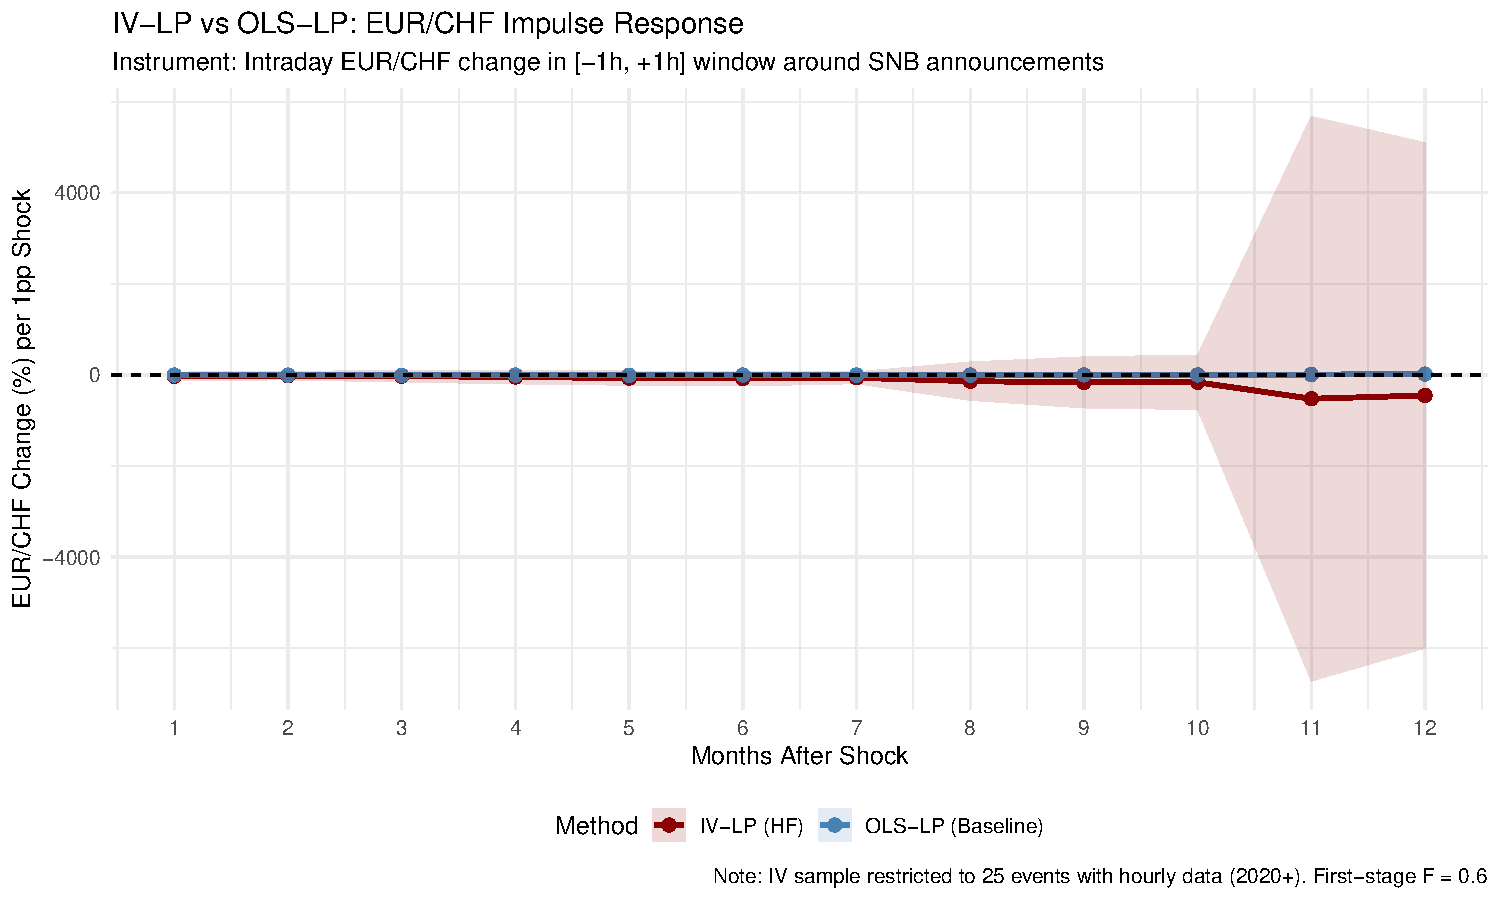
\includegraphics[width=\textwidth]{irf_hf_vs_baseline.pdf}
	\caption{IV-LP vs OLS-LP: EUR/CHF impulse response comparison. The IV estimates use intraday EUR/CHF changes as an instrument for the monetary policy shock.}
	\label{fig:hf_irf}
\end{figure}

% latex table generated in R 4.5.1 by xtable 1.8-4 package
% Tue Feb 10 16:28:37 2026
\begin{table}[ht]
\centering
\caption{First-Stage Regression: HF EUR/CHF Surprise as Instrument for MP Shock} 
\label{tab:hf_first_stage}
\begin{tabular}{lrrrr}
  \toprule
Variable & Estimate & SE & t.stat & p.value \\ 
  \midrule
(Intercept) & -0.0970 & (0.0731) & -1.33 & 0.200 \\ 
  hf\_surprise & 0.1279 & (0.1623) & 0.79 & 0.440 \\ 
  yield\_2y & 0.0604 & (0.0294) & 2.06 & 0.054 \\ 
  vix & 0.0004 & (0.0009) & 0.44 & 0.668 \\ 
  kof\_lag1 & 0.0012 & (0.0007) & 1.80 & 0.088 \\ 
  cpi\_yoy\_lag1 & -0.0229 & (0.0116) & -1.97 & 0.064 \\ 
   \bottomrule
\end{tabular}
\end{table}


% latex table generated in R 4.5.1 by xtable 1.8-4 package
% Tue Feb 10 15:47:33 2026
\begin{table}[ht]
\centering
\caption{IV-LP vs OLS-LP: EUR/CHF Response Comparison} 
\label{tab:irf_hf_comparison}
\begin{tabular}{crrrr}
  \toprule
horizon & coef fmt IV-LP (HF) & coef fmt OLS-LP (Baseline) & se fmt IV-LP (HF) & se fmt OLS-LP (Baseline) \\ 
  \midrule
  1 & -30.61 & -2.79 & (47.50) & (2.12) \\ 
    3 & -26.86 & -9.68*** & (66.92) & (1.89) \\ 
    6 & -79.30 & -3.62 & (82.95) & (3.25) \\ 
   12 & -451.07 & 17.48*** & (2831.50) & (5.02) \\ 
   \bottomrule
\end{tabular}
\end{table}


\subsection{Discussion}

The first-stage F-statistic of 0.62 falls well below the conventional threshold of 10 for instrument relevance \citep{stock2018}, classifying the intraday EUR/CHF surprise as a weak instrument. The coefficient on \texttt{hf\_surprise} in the first-stage regression is 0.128 with a standard error of 0.162 ($p = 0.44$), indicating that the hourly exchange rate movement around announcements is not a strong predictor of the monthly purging-regression residual.

This weak instrument problem has clear consequences for the second-stage IV-LP estimates. The IV coefficients are enormous in magnitude (e.g., $-451$ at $h=12$) with correspondingly massive standard errors (2,831), reflecting the well-known amplification of noise when the first stage is weak. By contrast, the OLS-LP baseline produces economically plausible estimates: a $-9.68\%$ response at $h=3$ (significant at 1\%) and a sign reversal to $+17.5\%$ at $h=12$.

The weakness of the instrument likely stems from two sources. First, the sample is restricted to 25 events from 2020 onward where hourly data is available---far too few observations for reliable IV estimation. Second, the hourly EUR/CHF change captures the immediate market reaction, which may not map linearly onto the monthly-frequency purging-regression residual that also absorbs information revealed between meetings.

\textbf{Implications for RQ1:} The failure of the IV strategy does not invalidate the baseline identification. Rather, it underscores the main thesis's acknowledgment that monthly-frequency purging regression faces identification constraints that high-frequency data could in principle resolve, but the available sample is insufficient. The qualitative finding that rate cuts depreciate the franc (negative OLS-LP coefficients at short horizons) remains the most reliable result. Future research with longer intraday samples could revisit this approach as a stronger cross-check.


% =========================================================================
% EXTENSION 2: SMOOTH TRANSITION LOCAL PROJECTIONS
% =========================================================================
\section{Smooth Transition Local Projections}\label{sec:smooth}

\subsection{Motivation}

The main analysis uses a hard regime dummy (positive vs.\ negative interest rates) to capture potential nonlinearities in monetary policy transmission. However, the transition between regimes is unlikely to be discrete. Following the smooth transition regression framework of \citet{auerbach2013} and \citet{tenreyro2016}, we replace the binary indicator with a logistic transition function that allows for gradual regime shifts. This addresses whether the large regime asymmetries documented in the main thesis---particularly the CPI differences driven by the 2015 floor removal---are robust to the specification of the regime boundary.

\subsection{Methodology}

Define the transition function:
\begin{equation}
	G(z_t; \gamma, c) = \frac{1}{1 + \exp\left(\gamma \cdot (z_t - c)\right)}
\end{equation}
where $z_t$ is the policy rate, $\gamma$ controls the transition speed (higher $\gamma$ approximates the hard threshold), and $c = 0\%$ is the threshold. The smooth transition LP is:
\begin{equation}
	\Delta y_{t+h} = \beta_h^{\text{low}} \cdot \text{mp\_shock}_t \cdot G(z_t) + \beta_h^{\text{high}} \cdot \text{mp\_shock}_t \cdot (1 - G(z_t)) + \boldsymbol{X}_t'\boldsymbol{\phi}_h + \varepsilon_{t+h}
\end{equation}

We estimate this for $\gamma \in \{1, 3, 5, 10\}$ to assess sensitivity to the transition speed.

\subsection{Results}

\begin{figure}[H]
	\centering
	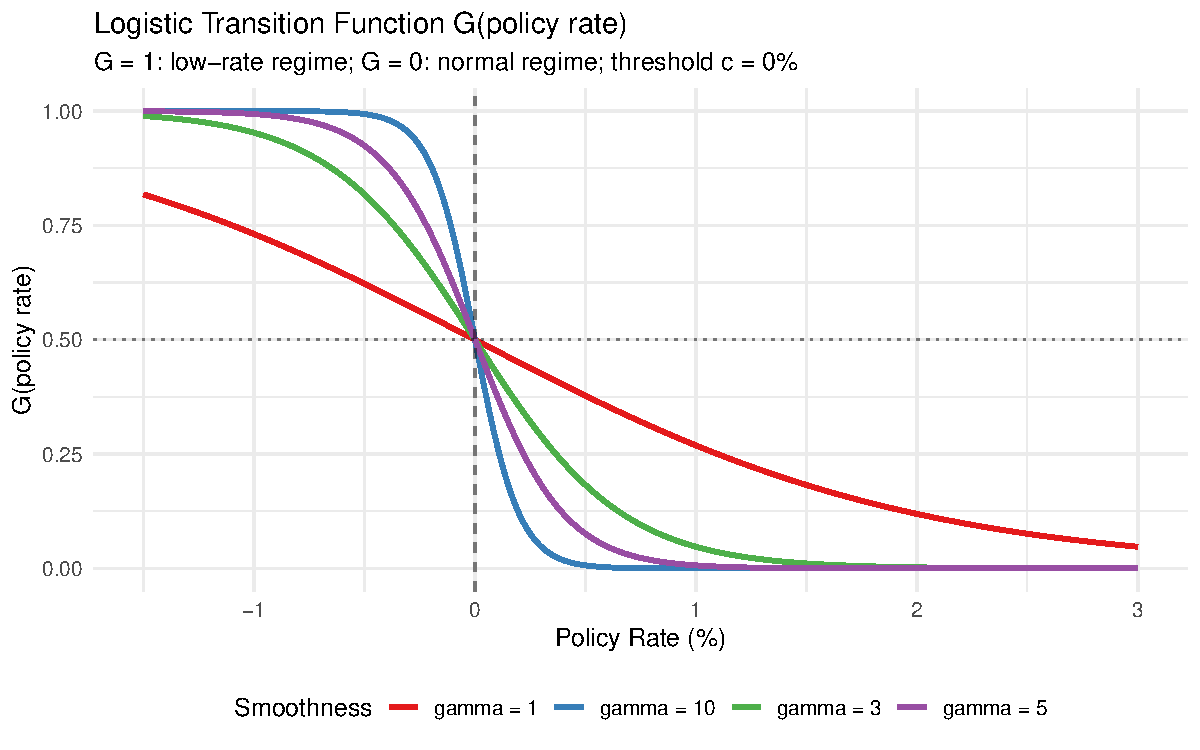
\includegraphics[width=0.7\textwidth]{transition_function.pdf}
	\caption{Logistic transition function $G(\text{policy rate})$ for different values of the smoothness parameter $\gamma$. Higher $\gamma$ approximates the hard regime dummy.}
	\label{fig:transition}
\end{figure}

\begin{figure}[H]
	\centering
	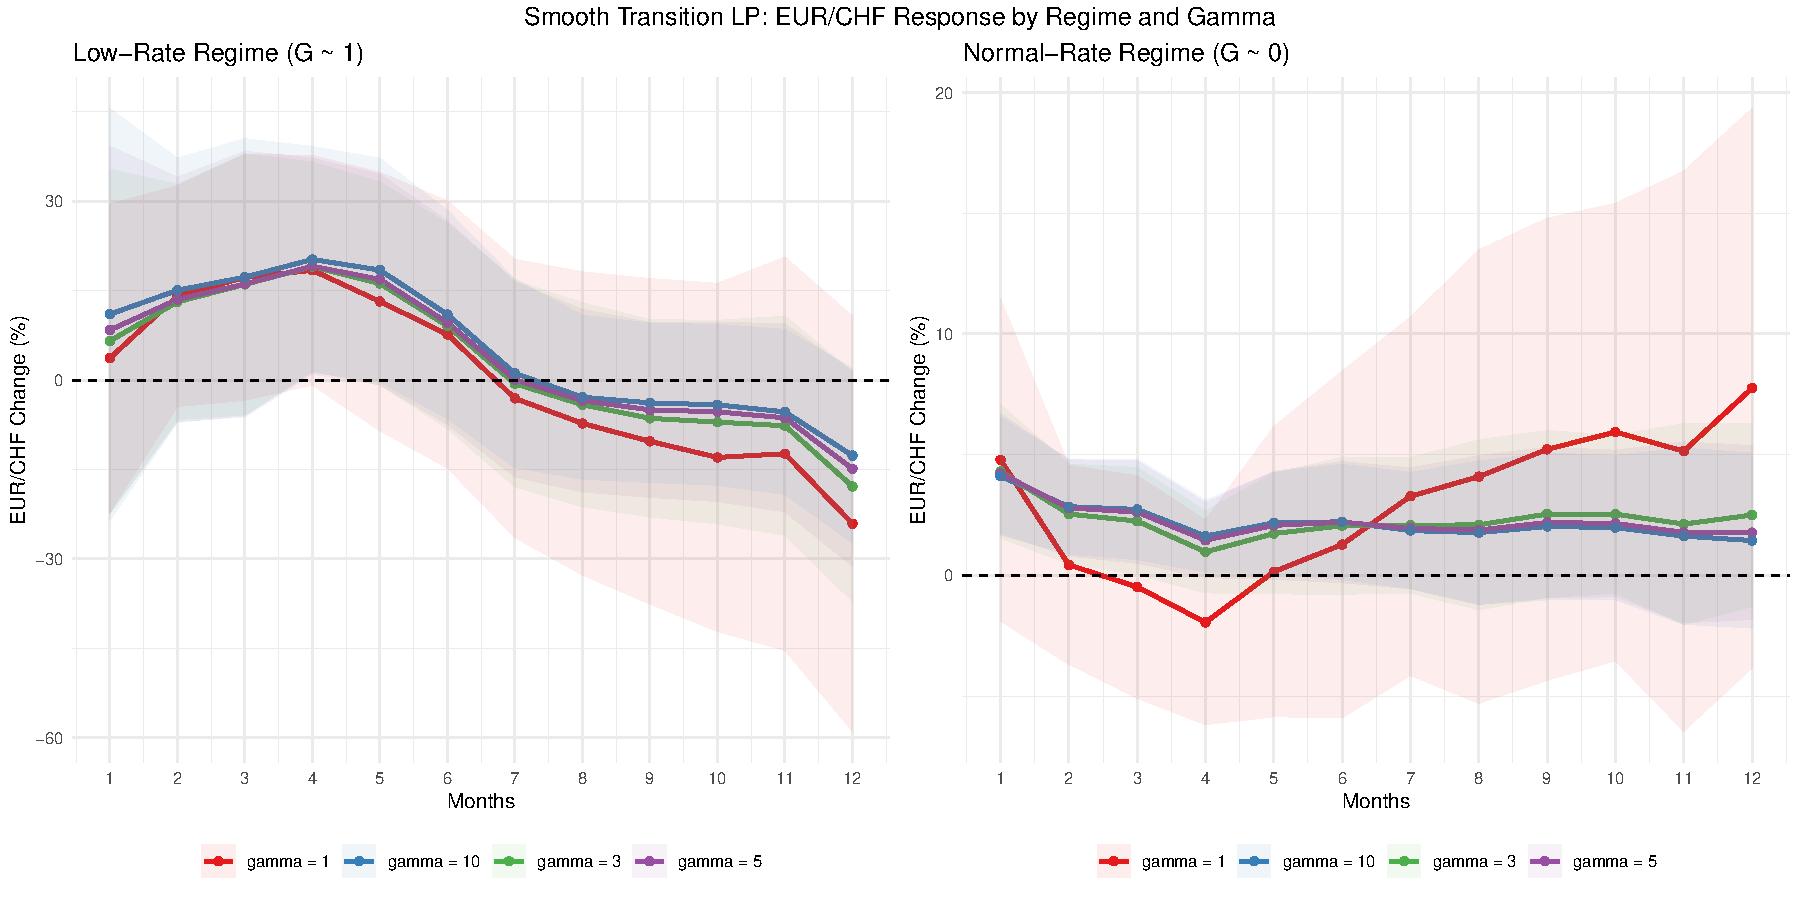
\includegraphics[width=\textwidth]{irf_smooth_transition_fx.pdf}
	\caption{Smooth transition LP: EUR/CHF impulse responses in the low-rate regime ($G \approx 1$) and normal-rate regime ($G \approx 0$) for different $\gamma$ values.}
	\label{fig:st_fx}
\end{figure}

\begin{figure}[H]
	\centering
	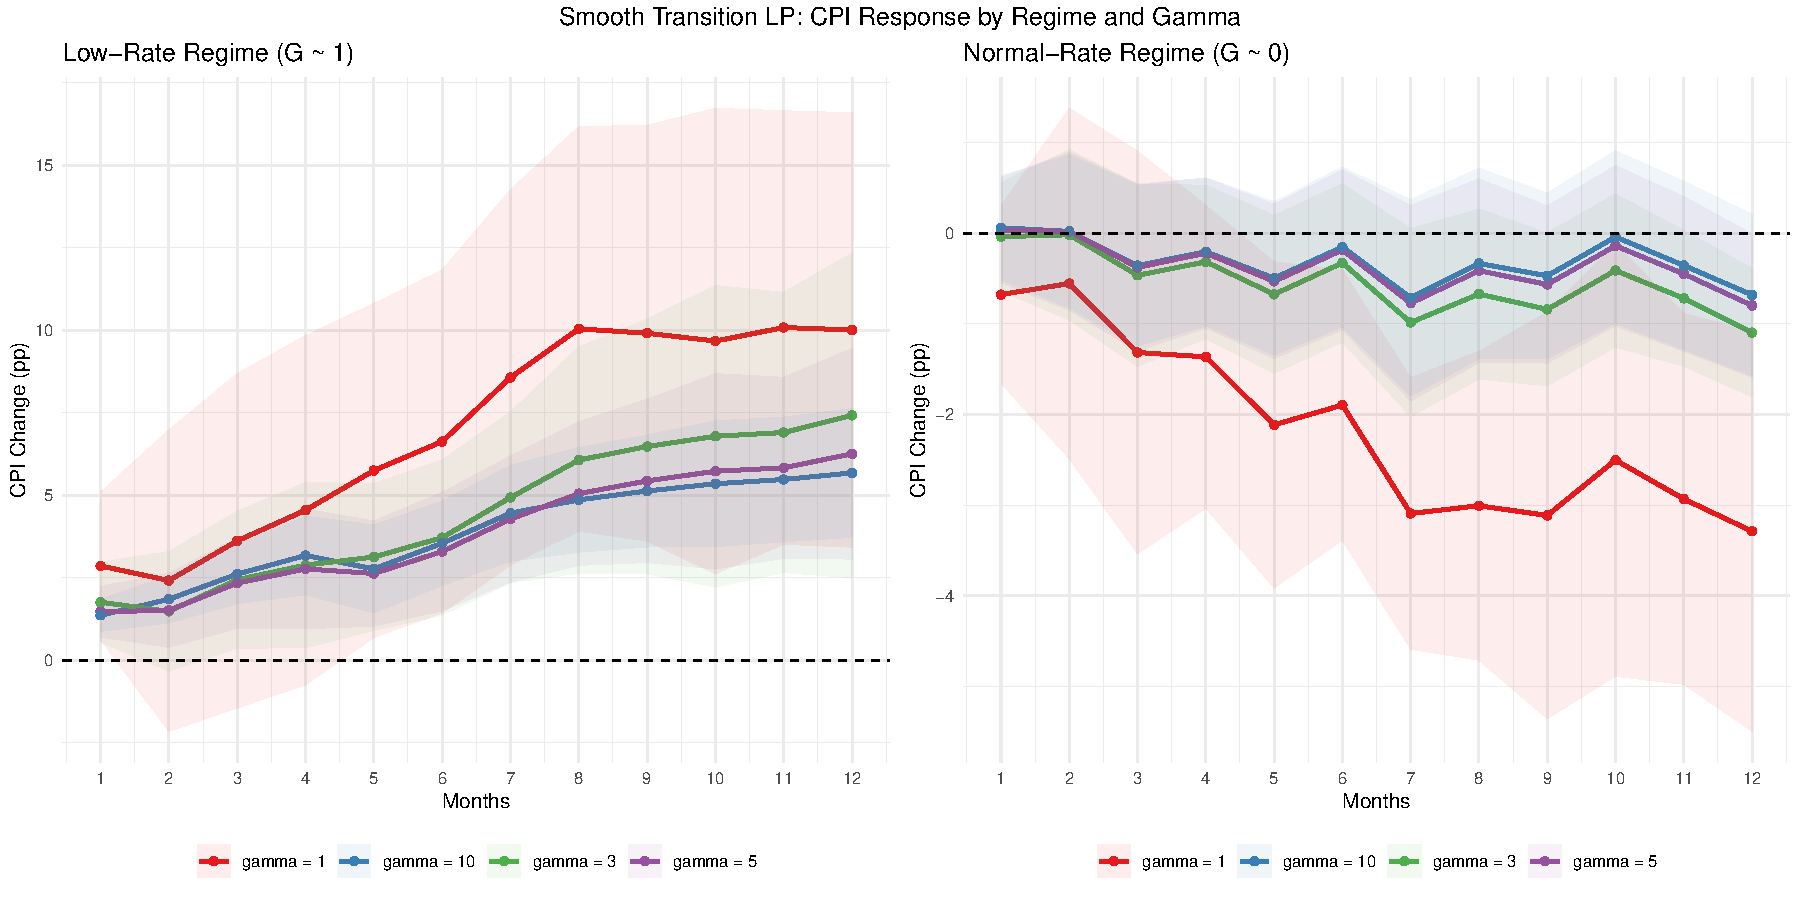
\includegraphics[width=\textwidth]{irf_smooth_transition_cpi.pdf}
	\caption{Smooth transition LP: CPI impulse responses by regime and transition speed.}
	\label{fig:st_cpi}
\end{figure}

% latex table generated in R 4.5.1 by xtable 1.8-4 package
% Tue Feb 10 15:50:00 2026
\begin{table}[ht]
\centering
\caption{Smooth Transition LP: EUR/CHF Response (gamma = 5, c = 0\%)} 
\label{tab:smooth_transition_results}
\begin{tabular}{crrr}
  \toprule
Horizon & Low-Rate Regime & Normal-Rate Regime & Difference \\ 
  \midrule
  1 & 8.39 (15.75) & 4.22 (1.26) & 4.17 \\ 
    3 & 16.11 (11.37) & 2.62 (1.08) & 13.49 \\ 
    6 & 9.63 (8.71) & 2.20 (1.28) & 7.43 \\ 
   12 & -14.89 (8.33) & 1.77 (1.84) & -16.66 \\ 
   \bottomrule
\end{tabular}
\end{table}


\subsection{Discussion}

The smooth transition results for the preferred specification ($\gamma = 5$) reveal a pattern consistent with the main thesis but with important nuances. In the normal-rate regime, EUR/CHF responses are precisely estimated and economically meaningful: a 4.22\% depreciation at $h=1$ (SE = 1.26), declining gradually to 1.77\% at $h=12$. These estimates closely match the pooled baseline from the main analysis (4.53\% at $h=1$), confirming that the exchange rate channel operates reliably when conventional policy tools are available.

In the low-rate regime, point estimates are substantially larger (8.39\% at $h=1$, peaking at 16.11\% at $h=3$) but with standard errors an order of magnitude wider (15.75 and 11.37, respectively). The sign reversal at $h=12$ ($-14.89$) mirrors the pattern found in the hard-threshold regime analysis. This imprecision reflects the fundamental constraint identified in the main thesis: only two negative-rate cuts exist in the sample, both coinciding with the January 2015 EUR/CHF floor removal.

A key finding emerges from comparing across $\gamma$ values: the normal-rate regime coefficients are stable across all transition speeds, while low-rate coefficients vary substantially. This confirms that the regime asymmetry is driven by a small number of extreme observations rather than a smooth structural shift in the transmission mechanism. As $\gamma$ decreases (smoother transition), the low-rate estimates become less extreme because more moderate observations receive partial low-rate weight, diluting the influence of the 2015 episode.

\textbf{Implications for RQ1:} The stable normal-rate estimates across $\gamma$ values strengthen confidence in the core finding of approximately 4\% depreciation per pp shock. The instability of low-rate estimates across $\gamma$ values supports the main thesis's cautious interpretation that negative-rate regime differences reflect the 2015 floor removal rather than a fundamental shift in monetary transmission. For RQ2, the DSGE model's prediction of minimal regime differences (+0.02pp inflation) aligns better with the smooth transition framework's suggestion that regime boundaries are not structurally sharp.


% =========================================================================
% EXTENSION 3: WILD BOOTSTRAP CONFIDENCE INTERVALS
% =========================================================================
\section{Wild Bootstrap Confidence Intervals}\label{sec:bootstrap}

\subsection{Motivation}

Local projection standard errors are typically computed using the \citet{newey1987} heteroskedasticity and autocorrelation consistent (HAC) estimator. However, HAC inference can perform poorly in small samples, which is relevant for our analysis given the limited number of policy rate changes (19 cuts in 300 months). The Rademacher wild bootstrap provides an alternative that has better finite-sample properties \citep{gonccalves2004}. This is particularly important given the main thesis's acknowledgment that small sample size severely constrains the analysis.

\subsection{Methodology}

For each horizon $h$:
\begin{enumerate}
	\item Estimate the baseline LP and compute the observed $t$-statistic for the shock coefficient.
	\item Under $H_0: \beta_h = 0$, estimate the restricted model and obtain fitted values $\hat{y}_t^r$ and residuals $\hat{e}_t^r$.
	\item For $b = 1, \ldots, B$ (with $B = 999$):
	\begin{itemize}
		\item Draw Rademacher weights $w_t \in \{-1, +1\}$ with equal probability.
		\item Construct bootstrap outcome: $y_t^{*} = \hat{y}_t^r + \hat{e}_t^r \cdot w_t$.
		\item Estimate the LP on bootstrap data and compute the bootstrap $t$-statistic $t_b^*$.
	\end{itemize}
	\item The bootstrap $p$-value is $\hat{p} = B^{-1} \sum_{b=1}^{B} \mathbf{1}(|t_b^*| \geq |t_{\text{obs}}|)$.
	\item Percentile-$t$ bootstrap CIs: $[\hat{\beta} - q_{0.975}^* \cdot \hat{\sigma}, \; \hat{\beta} - q_{0.025}^* \cdot \hat{\sigma}]$.
\end{enumerate}

\subsection{Results}

\begin{figure}[H]
	\centering
	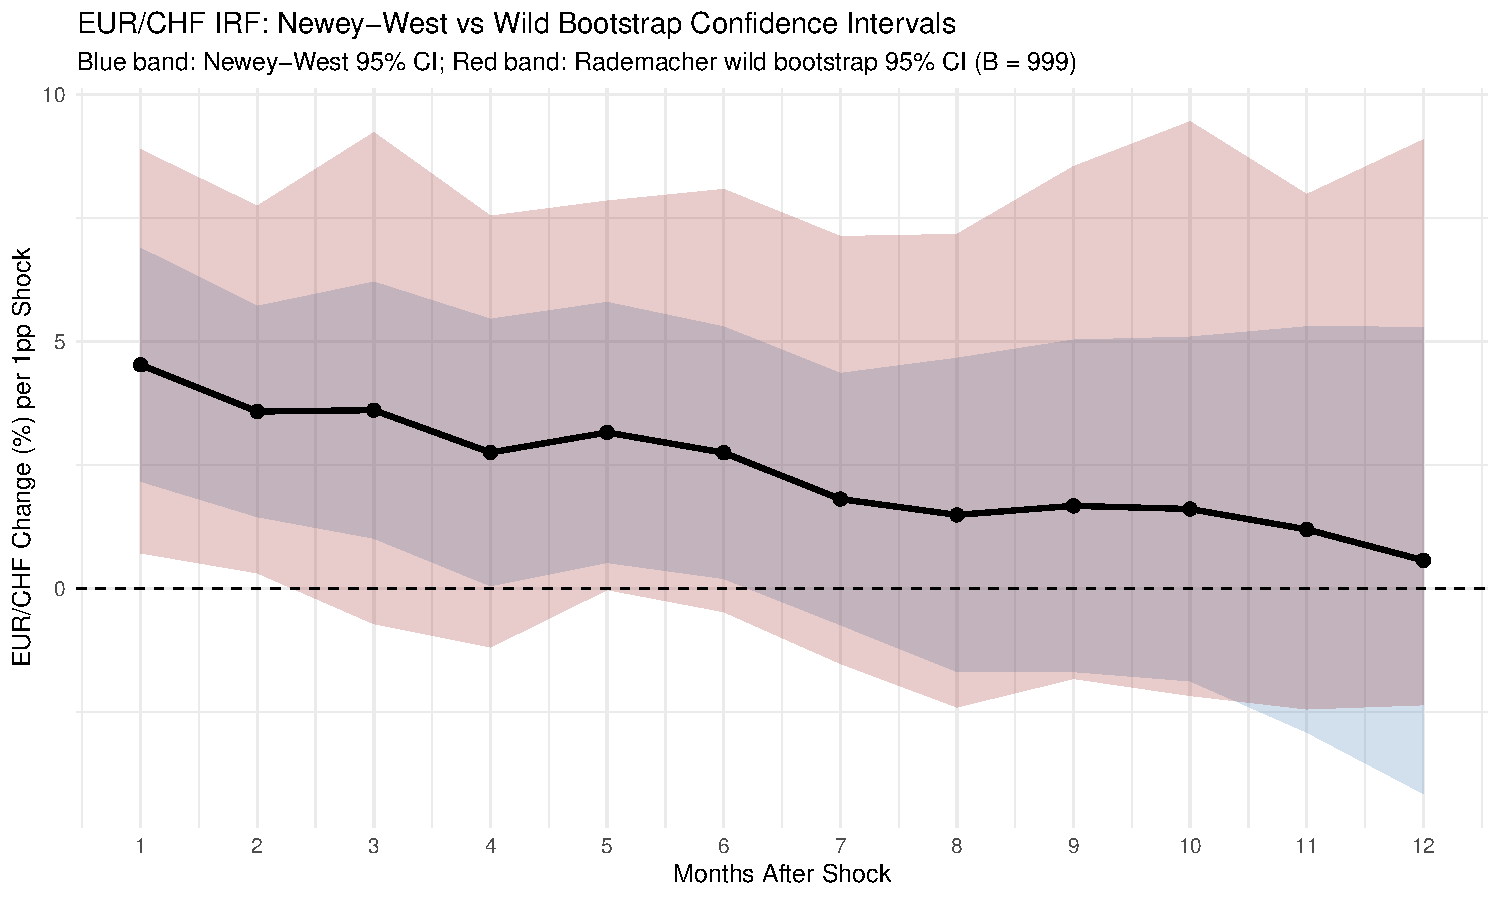
\includegraphics[width=\textwidth]{irf_bootstrap_fx.pdf}
	\caption{EUR/CHF IRF with Newey-West (blue) and wild bootstrap (red) 95\% confidence intervals.}
	\label{fig:boot_fx}
\end{figure}

\begin{figure}[H]
	\centering
	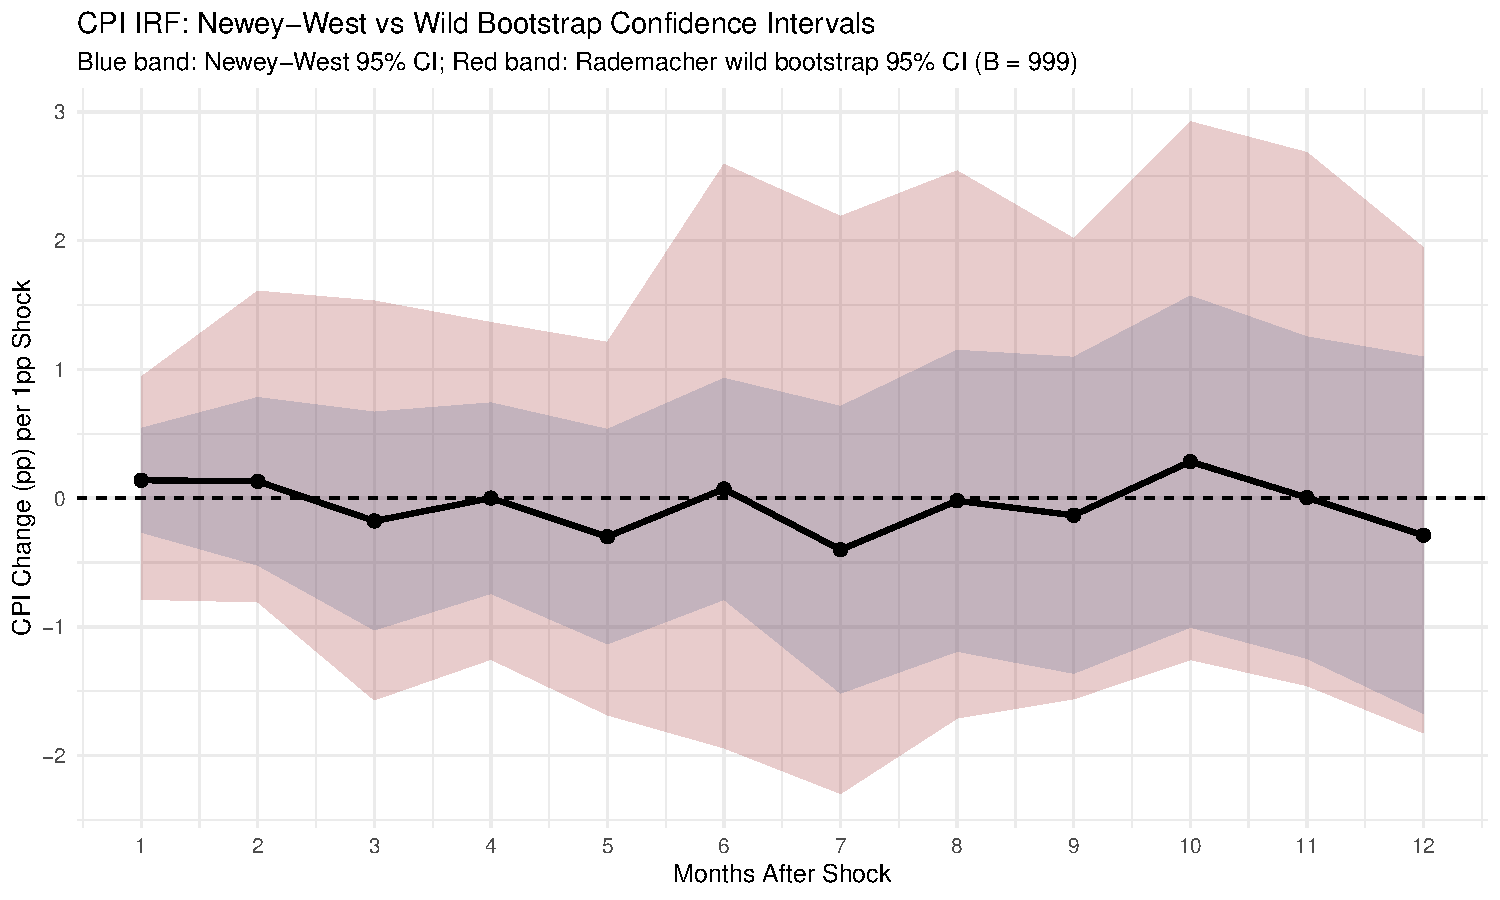
\includegraphics[width=\textwidth]{irf_bootstrap_cpi.pdf}
	\caption{CPI IRF with Newey-West and wild bootstrap confidence intervals.}
	\label{fig:boot_cpi}
\end{figure}

% latex table generated in R 4.5.1 by xtable 1.8-4 package
% Tue Feb 10 09:28:51 2026
\begin{table}[ht]
\centering
\caption{Wild Bootstrap vs Newey-West: EUR/CHF Response (B = 999)} 
\label{tab:bootstrap_comparison}
\begin{tabular}{crcrcr}
  \toprule
Horizon & Coeff. & NW 95\% CI & NW p-val & Bootstrap 95\% CI & Boot. p-val \\ 
  \midrule
  1 & 4.53 & [2.17, 6.89] & 0.000 & [0.72, 8.88] & 0.025 \\ 
    3 & 3.61 & [1.02, 6.20] & 0.006 & [-0.71, 9.23] & 0.128 \\ 
    6 & 2.75 & [0.20, 5.30] & 0.034 & [-0.47, 8.08] & 0.293 \\ 
   12 & 0.57 & [-4.15, 5.29] & 0.813 & [-2.36, 9.08] & 0.848 \\ 
   \bottomrule
\end{tabular}
\end{table}


\subsection{Discussion}

The bootstrap analysis yields a clear hierarchy of statistical significance across horizons. At $h=1$, the EUR/CHF depreciation of 4.53\% remains statistically significant under the wild bootstrap ($p = 0.025$), though the confidence interval widens from $[2.17, 6.89]$ (Newey-West) to $[0.72, 8.88]$ (bootstrap). This confirms the impact effect as the most robust finding.

At $h=3$, the result that appeared highly significant under Newey-West ($p = 0.006$) loses significance under the bootstrap ($p = 0.128$), with the confidence interval expanding from $[1.02, 6.20]$ to $[-0.71, 9.23]$ and now including zero. Similarly, the $h=6$ result ($p_{\text{NW}} = 0.034$ vs.\ $p_{\text{boot}} = 0.293$) is no longer significant. At $h=12$, both methods agree on insignificance.

The pattern of wider bootstrap CIs is consistent with the theoretical expectation that Newey-West approximations are optimistic in small samples. The asymmetric widening---bootstrap CIs shift upward relative to Newey-West---suggests that the $t$-statistic distribution under the null is left-skewed, which HAC standard errors do not capture.

\textbf{Implications for RQ1:} The bootstrap results refine the main thesis's answer to RQ1 regarding exchange rates. The \emph{impact} depreciation effect (approximately 4.5\% at $h=1$) is robust to inference method, but the \emph{persistence} of the effect (significant through $h=6$ under Newey-West) should be interpreted more cautiously. The conservative conclusion is that SNB rate cuts generate a significant immediate franc depreciation, with suggestive but not statistically robust evidence of persistence beyond 1 month. For CPI, both inference methods agree on the absence of significant pooled effects, strengthening the main finding of weak inflation pass-through. This aligns with the DSGE model's prediction of muted CPI responses due to incomplete exchange rate pass-through and habit formation (RQ2).


% =========================================================================
% EXTENSION 4: PLACEBO / FALSIFICATION TESTS
% =========================================================================
\section{Placebo and Falsification Tests}\label{sec:placebo}

\subsection{Motivation}

A well-identified monetary policy shock should only produce significant effects when actual policy changes occur. If the same LP specification yields significant results when applied to ``no-change'' meetings where the SNB held rates constant, this would cast doubt on the identification strategy \citep{ramey2016}. This extension directly addresses the main thesis's concern that the purging regression may not adequately separate anticipated from unanticipated policy actions.

\subsection{Methodology}

We construct two types of placebo tests:

\begin{enumerate}
	\item \textbf{Fitted-value placebo}: On meeting dates where $\Delta r_t = 0$ (68 hold decisions), we use the predicted component from the purging regression (i.e., the fitted value $\hat{\Delta r}_t$, representing the anticipated policy action) as a ``shock.'' If identification is valid, anticipated actions should not produce significant exchange rate or inflation responses.

	\item \textbf{Permutation test}: We randomly shuffle the shock assignment across time periods ($N = 500$ permutations) and re-estimate the LPs. The permutation $p$-value is the fraction of randomized coefficients exceeding the actual estimate in absolute value.
\end{enumerate}

\subsection{Results}

\begin{figure}[H]
	\centering
	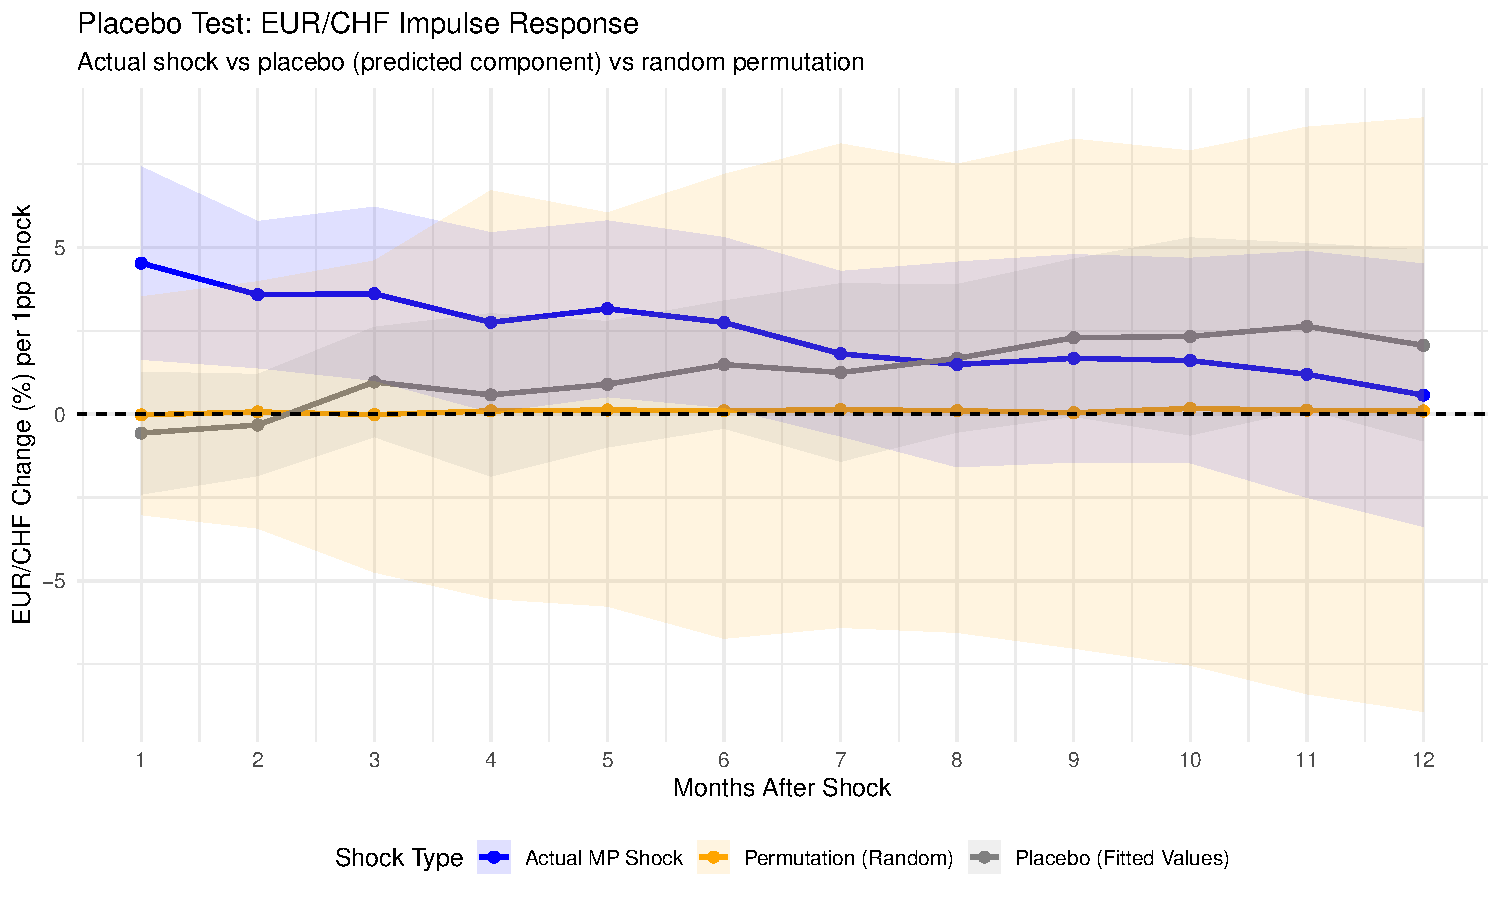
\includegraphics[width=\textwidth]{placebo_fx.pdf}
	\caption{Placebo test for EUR/CHF: actual shock vs.\ placebo (fitted values) vs.\ random permutation.}
	\label{fig:placebo_fx}
\end{figure}

\begin{figure}[H]
	\centering
	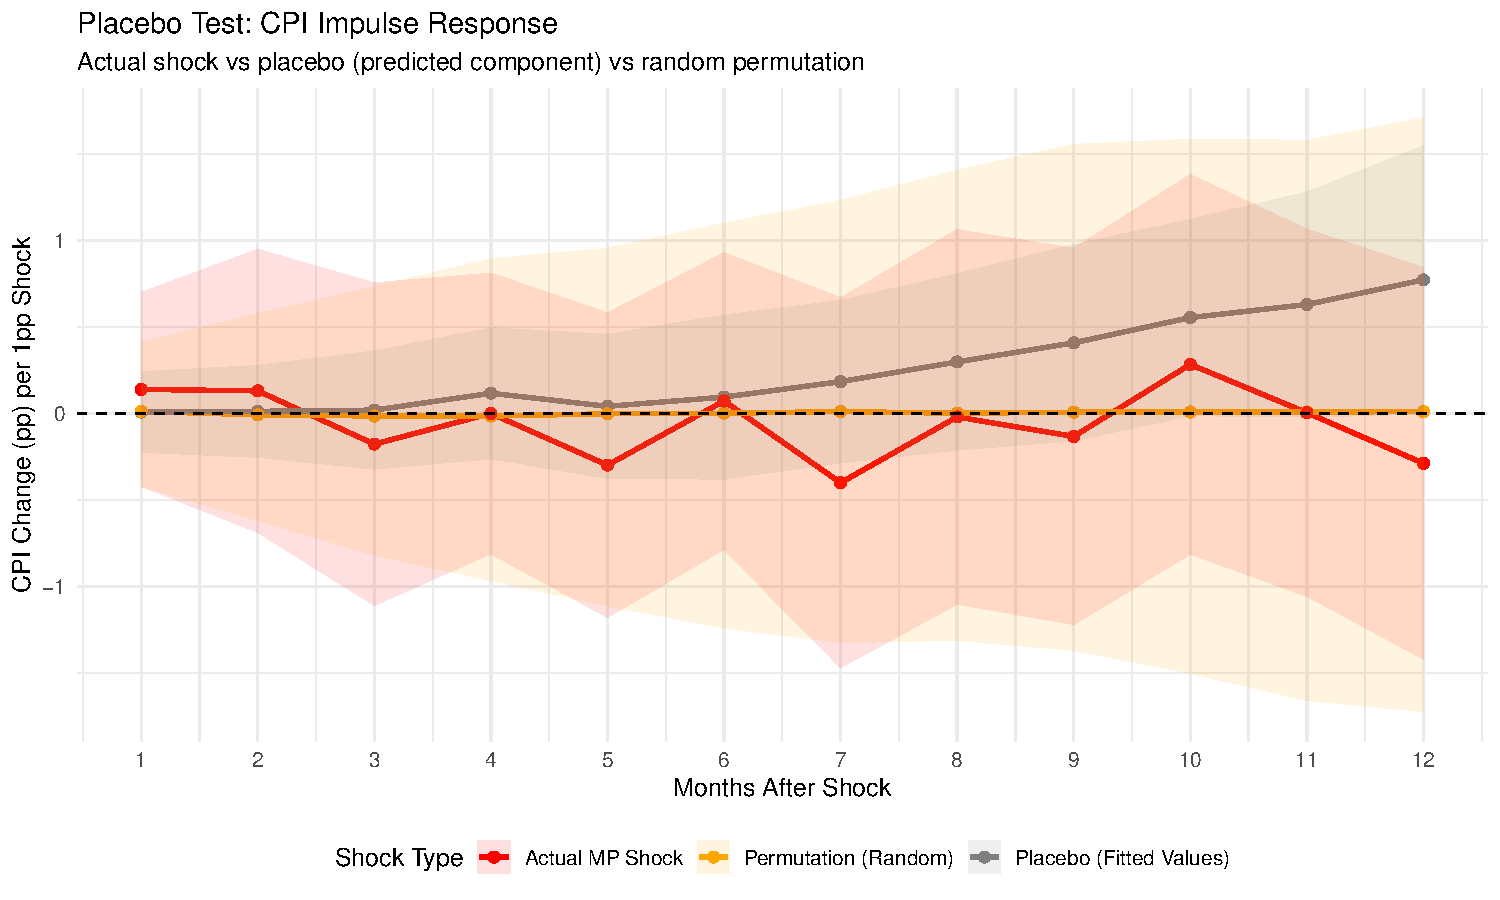
\includegraphics[width=\textwidth]{placebo_cpi.pdf}
	\caption{Placebo test for CPI: actual shock vs.\ placebo vs.\ random permutation.}
	\label{fig:placebo_cpi}
\end{figure}

% latex table generated in R 4.5.1 by xtable 1.8-4 package
% Tue Feb 10 16:39:33 2026
\begin{table}[ht]
\centering
\caption{Placebo and Permutation Tests: Comparison of Responses} 
\label{tab:placebo_results}
\begin{tabular}{lrrrr}
  \toprule
Variable & h = 1 & h = 3 & h = 6 & h = 12 \\ 
  \midrule
Actual (FX) & 4.53 & 3.61 & 2.75 & 0.57 \\ 
  Placebo (FX) & -0.57 & 0.97 & 1.49 & 2.06 \\ 
  Perm.~p (FX) & 0.018 & 0.116 & 0.344 & 0.878 \\ 
  Actual (CPI) & 0.14 & -0.18 & 0.07 & -0.29 \\ 
  Placebo (CPI) & 0.01 & 0.02 & 0.09 & 0.77 \\ 
  Perm.~p (CPI) & 0.544 & 0.654 & 0.908 & 0.750 \\ 
   \bottomrule
\end{tabular}
\end{table}


\subsection{Discussion}

The placebo tests provide strong support for the identification strategy at short horizons but weaker support as the horizon increases. Three key results emerge.

First, the placebo shock coefficients are close to zero and economically negligible at all horizons for both EUR/CHF ($-0.57$ at $h=1$) and CPI ($0.01$ at $h=1$), compared with actual shock effects of 4.53 and 0.14, respectively. The predicted component of policy---which captures the systematic response to macroeconomic conditions---does not generate exchange rate movements, confirming that the purging regression successfully removes this anticipated component.

Second, the permutation test rejects the null at $h=1$ for EUR/CHF with $p = 0.018$: only 1.8\% of random shock assignments produce coefficients as large as the actual estimate. This provides direct evidence that the observed impact depreciation is unlikely to arise by chance. However, permutation $p$-values increase rapidly with the horizon ($p = 0.116$ at $h=3$, $p = 0.344$ at $h=6$, $p = 0.878$ at $h=12$), consistent with the bootstrap finding that persistence beyond impact is statistically fragile.

Third, for CPI, permutation $p$-values are uniformly large (0.544 to 0.908), consistent with the main finding that pooled inflation responses are indistinguishable from zero.

\textbf{Implications for RQ1 and RQ2:} The placebo results strengthen the causal interpretation of the impact exchange rate effect. The fact that anticipated policy (fitted values) generates no response while unanticipated policy (residuals) generates a 4.5\% depreciation is precisely what a correctly identified shock should produce. This addresses the main thesis's concern about identification constraints: at least at $h=1$, the purging regression appears to isolate genuine policy surprises. The declining permutation significance at longer horizons is consistent with the bootstrap results and suggests that the true causal effect is concentrated at impact. For CPI, the absence of significant placebo or permutation results is uninformative---it is consistent with both correct identification (no true CPI effect) and incorrect identification (both actual and placebo shocks miss the true channel).


% =========================================================================
% EXTENSION 5: INFORMATION EFFECTS
% =========================================================================
\section{Information Effects}\label{sec:info}

\subsection{Motivation}

Central bank announcements convey not only policy actions but also information about the central bank's assessment of economic conditions. \citet{nakamura2018} and \citet{jarocinski2020} show that disentangling ``pure monetary policy'' from ``information'' components is crucial for correctly identifying transmission mechanisms. The main thesis explicitly acknowledges information effects as a key limitation of the purging regression approach, noting that monthly frequency prevents separating these channels. This extension provides a first attempt at doing so with the available data.

\subsection{Methodology}

We classify each nonzero MP shock month based on the co-movement of the shock and the one-month change in the 2-year government bond yield:
\begin{itemize}
	\item \textbf{Pure MP shock}: $\text{mp\_shock}_t$ and $\Delta \text{yield\_2y}_t$ have the same sign (easing lowers yields, tightening raises yields).
	\item \textbf{Information shock}: $\text{mp\_shock}_t$ and $\Delta \text{yield\_2y}_t$ have opposite signs (market revises expectations about the economy).
\end{itemize}

We then create separate shock variables and estimate:
\begin{equation}
	\Delta y_{t+h} = \beta_h^{\text{MP}} \cdot \text{shock}^{\text{pure}}_t + \beta_h^{\text{info}} \cdot \text{shock}^{\text{info}}_t + \boldsymbol{X}_t'\boldsymbol{\phi}_h + \varepsilon_{t+h}
\end{equation}

\subsection{Results}

\begin{figure}[H]
	\centering
	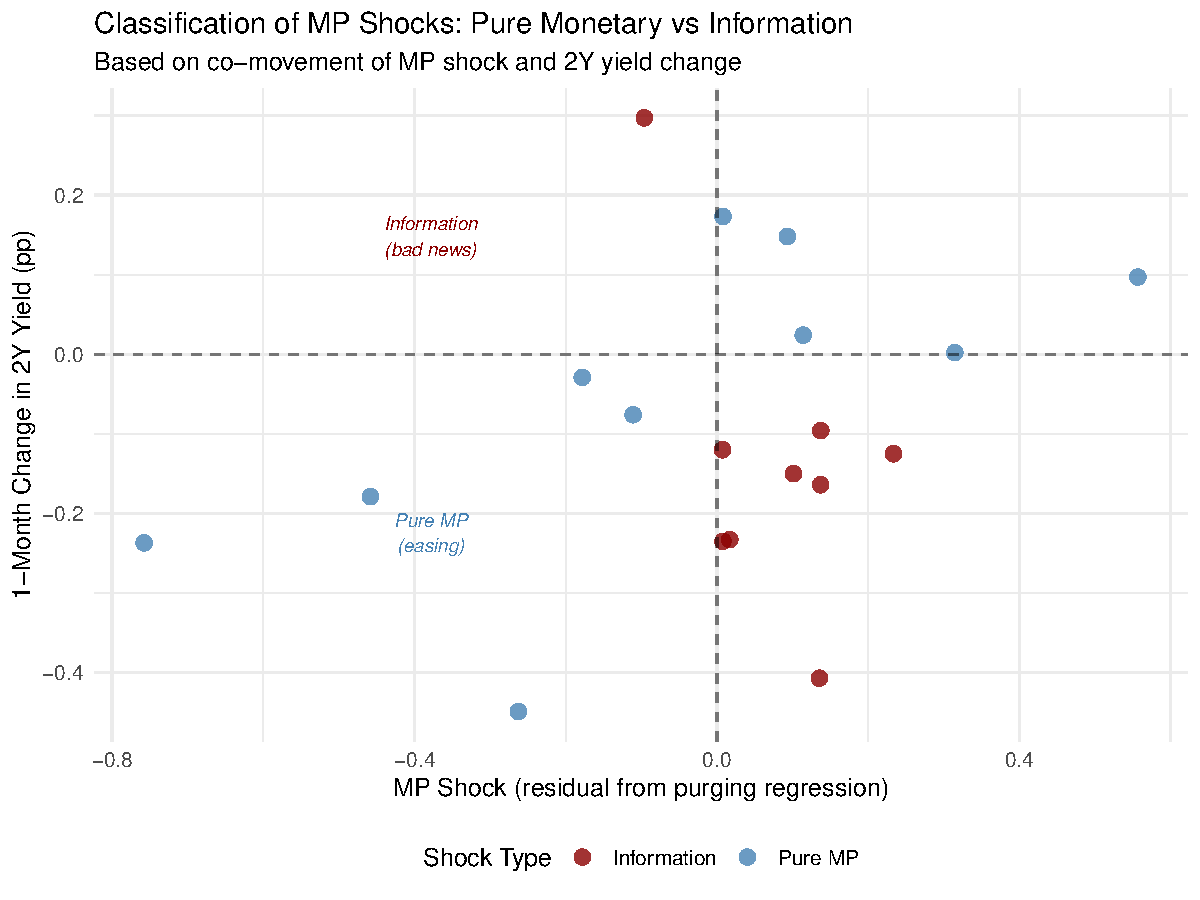
\includegraphics[width=0.85\textwidth]{info_vs_mp_classification.pdf}
	\caption{Classification of MP shocks into pure monetary and information components based on yield co-movement.}
	\label{fig:info_classify}
\end{figure}

\begin{figure}[H]
	\centering
	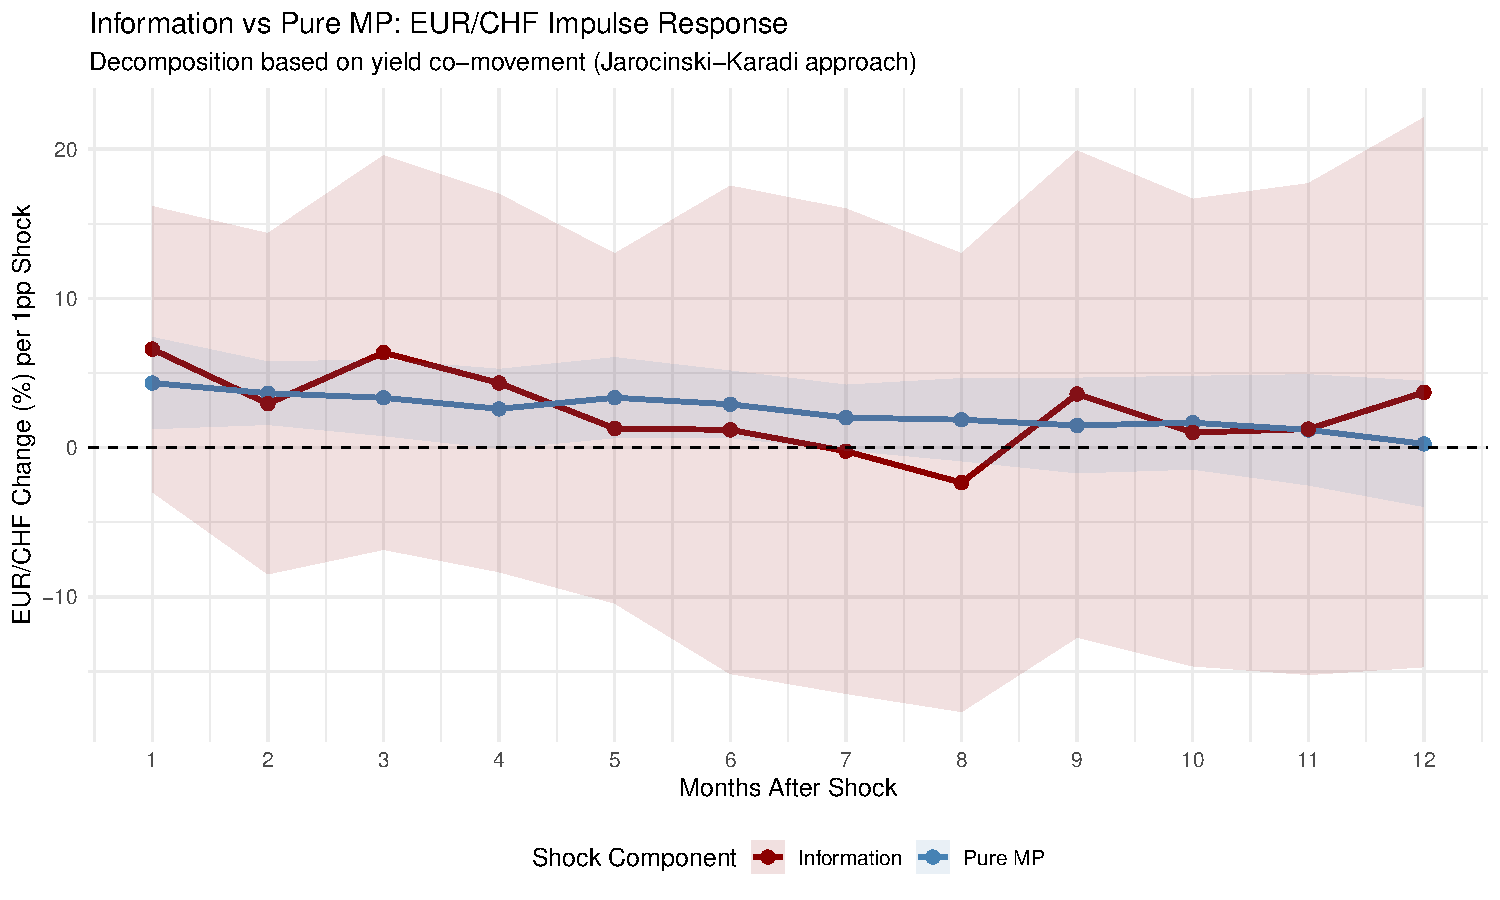
\includegraphics[width=\textwidth]{irf_info_vs_mp_fx.pdf}
	\caption{EUR/CHF impulse responses: pure MP shocks vs.\ information shocks.}
	\label{fig:info_fx}
\end{figure}

\begin{figure}[H]
	\centering
	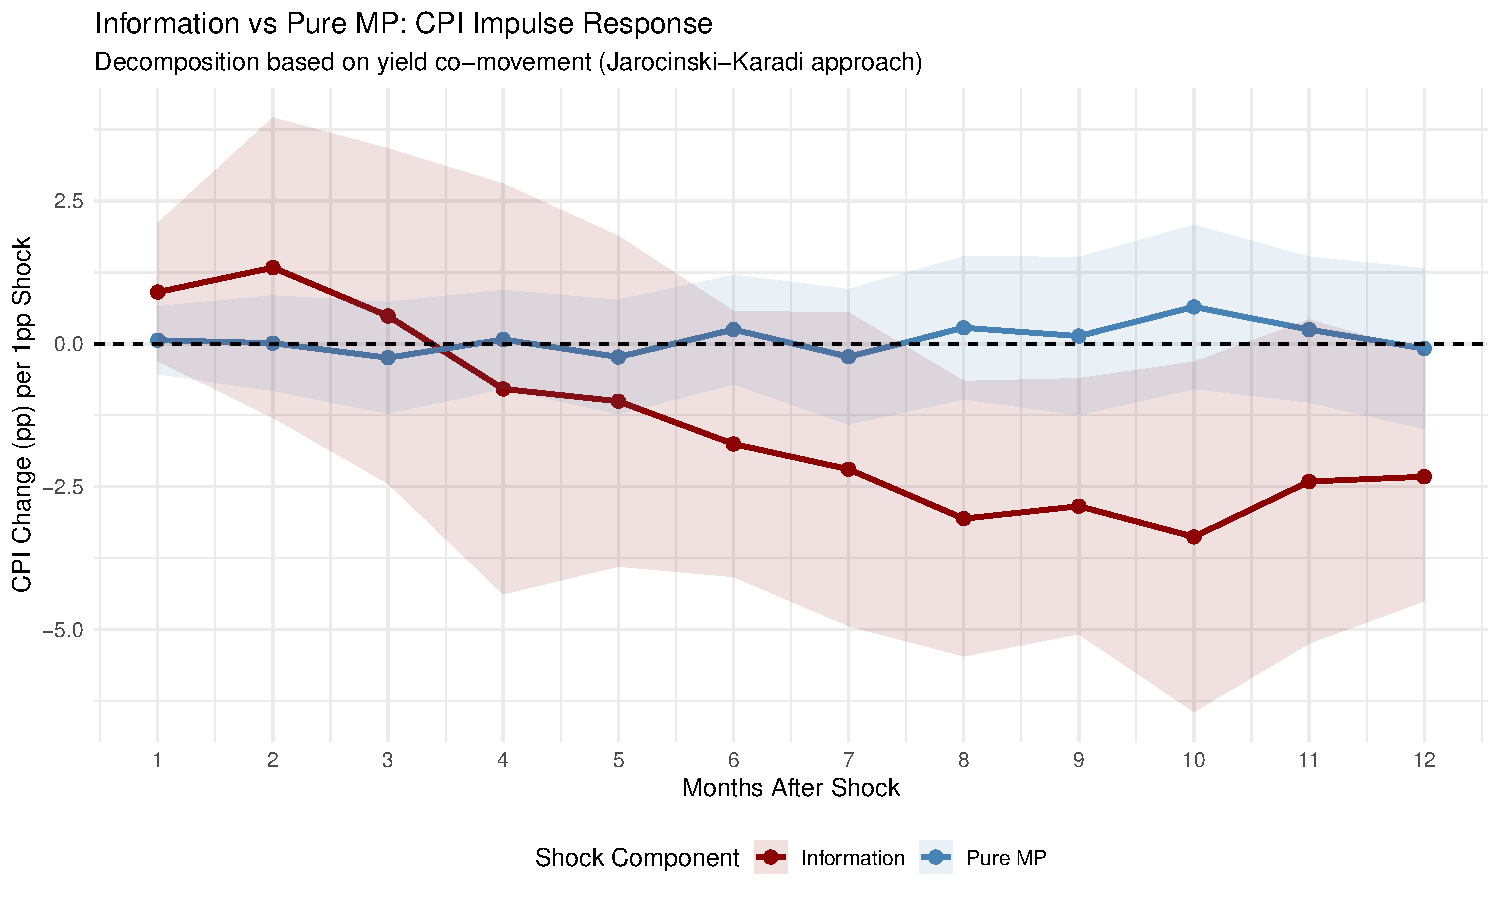
\includegraphics[width=\textwidth]{irf_info_vs_mp_cpi.pdf}
	\caption{CPI impulse responses: pure MP shocks vs.\ information shocks.}
	\label{fig:info_cpi}
\end{figure}

% latex table generated in R 4.5.1 by xtable 1.8-4 package
% Tue Feb 10 09:29:06 2026
\begin{table}[ht]
\centering
\caption{Information vs Pure MP Shocks: IRF Comparison} 
\label{tab:info_effects_results}
\begin{tabular}{clrr}
  \toprule
Horizon & Component & EUR/CHF & CPI \\ 
  \midrule
1.00 & Pure MP & 4.33 (1.56) & 0.06 (0.30) \\ 
  3.00 & Pure MP & 3.34 (1.30) & -0.24 (0.50) \\ 
  6.00 & Pure MP & 2.90 (1.14) & 0.25 (0.49) \\ 
  12.00 & Pure MP & 0.25 (2.14) & -0.08 (0.71) \\ 
  1.00 & Information & 6.60 (4.87) & 0.91 (0.61) \\ 
  3.00 & Information & 6.37 (6.73) & 0.49 (1.49) \\ 
  6.00 & Information & 1.19 (8.33) & -1.75 (1.18) \\ 
  12.00 & Information & 3.70 (9.38) & -2.32 (1.11) \\ 
   \bottomrule
\end{tabular}
\end{table}


\subsection{Discussion}

The decomposition reveals meaningful differences between pure monetary and information shocks across both outcome variables.

For EUR/CHF, information shocks generate a larger immediate depreciation (6.60\% at $h=1$) than pure MP shocks (4.33\%), but the dynamics differ sharply. Pure MP effects are persistent: the 4.33\% impact declines gradually to 2.90\% at $h=6$ before fading to 0.25\% at $h=12$. Information effects are front-loaded but less persistent: 6.60\% at impact, still 6.37\% at $h=3$, but dropping to 1.19\% at $h=6$ before partially rebounding to 3.70\% at $h=12$. The larger information shock impact is consistent with the \citet{nakamura2018} finding that ``Fed information effects'' amplify immediate asset price responses because markets are simultaneously updating their beliefs about both the policy stance and the economic outlook.

For CPI, the decomposition is more informative. Pure MP shocks generate essentially zero inflation responses at all horizons (ranging from $-0.24$ to $+0.25$ pp), consistent with the main thesis's finding of weak pooled pass-through. Information shocks, by contrast, produce a positive impact ($+0.91$ pp at $h=1$) that turns sharply negative at medium horizons ($-1.75$ pp at $h=6$, $-2.32$ pp at $h=12$). This sign reversal is economically intuitive: when the SNB cuts rates while markets learn negative economic news (the information channel), the initial inflationary impulse from depreciation is eventually dominated by the disinflationary effect of weaker economic conditions revealed by the central bank's action.

\textbf{Implications for RQ1 and RQ2:} The decomposition suggests that the baseline pooled estimates represent a weighted average of two distinct channels. The pure MP component---which is conceptually closest to what the DSGE model captures---produces exchange rate effects of approximately 4.3\%, closely matching the model's prediction of moderate depreciation. The near-zero CPI response to pure MP shocks validates the DSGE model's incomplete pass-through mechanism even more strongly than the pooled results. For RQ2, this is encouraging: the model's structural parameters (9\% immediate pass-through) appear well-calibrated to the pure monetary channel. The information channel, which the DSGE framework does not model, operates through a fundamentally different mechanism---belief updating about economic fundamentals rather than interest rate arbitrage.

An important caveat applies: this classification uses monthly yield changes rather than the intraday movements employed by \citet{jarocinski2020}, introducing substantial measurement noise. The results should be interpreted as suggestive of the importance of information effects in SNB communication rather than as precise quantitative estimates.


% =========================================================================
% EXTENSION 6: ADDITIONAL OUTCOME VARIABLES
% =========================================================================
\section{Additional Outcome Variables}\label{sec:outcomes}

\subsection{Motivation}

The main analysis focuses on EUR/CHF exchange rate and CPI inflation responses. To provide a more complete picture of the monetary transmission mechanism---and to test additional predictions of the DSGE model---we extend the LP framework to additional variables representing the yield curve channel (2-year and 10-year government bond yields) and real economic expectations (KOF Economic Barometer).

\subsection{Methodology}

For each additional outcome $y_t \in \{\text{yield\_2y}, \text{yield\_10y}, \text{kof}\}$, we estimate:
\begin{equation}
	y_{t+h} - y_t = \beta_h \cdot \text{mp\_shock}_t + \boldsymbol{X}_t'\boldsymbol{\phi}_h + \varepsilon_{t+h}, \quad h = 1, \ldots, 12
\end{equation}
using Newey-West standard errors with lag truncation $h$.

\subsection{Results}

\begin{figure}[H]
	\centering
	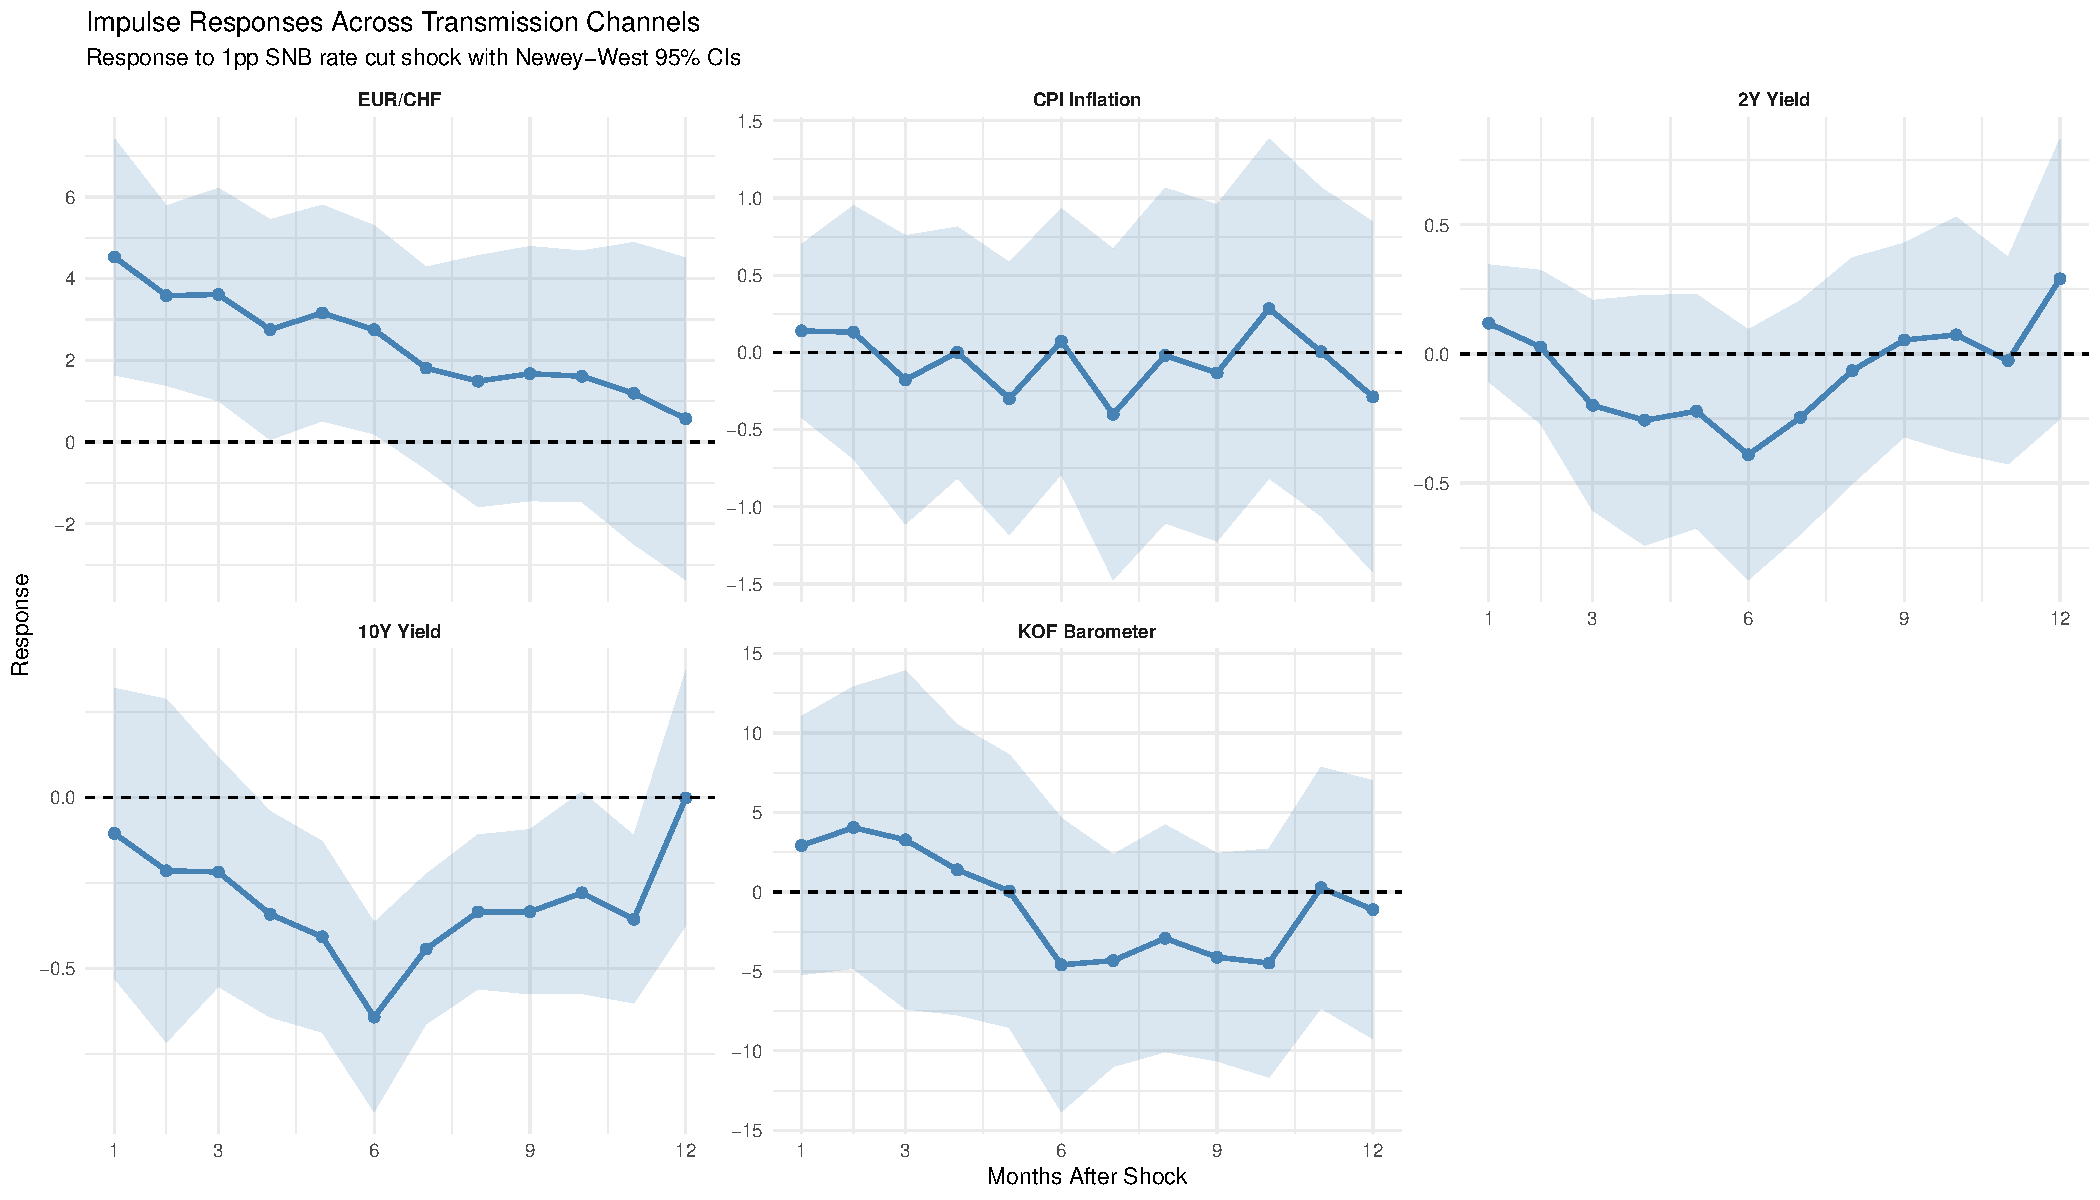
\includegraphics[width=\textwidth]{irf_all_outcomes.pdf}
	\caption{Multi-panel impulse responses across all transmission channels: EUR/CHF, CPI, 2Y yield, 10Y yield, and KOF barometer.}
	\label{fig:all_outcomes}
\end{figure}

\begin{figure}[H]
	\centering
	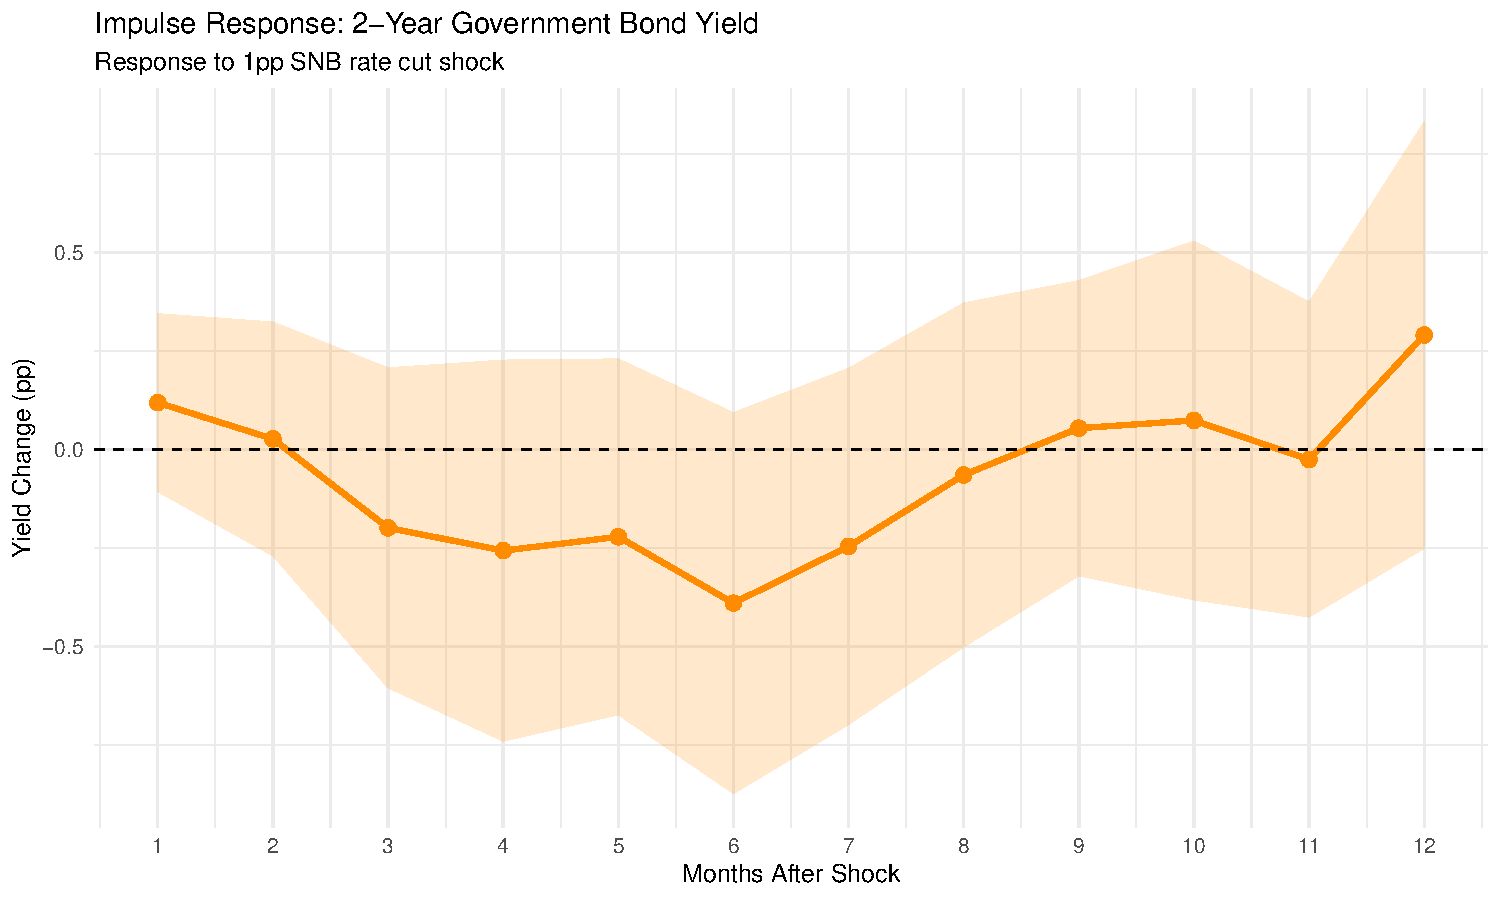
\includegraphics[width=\textwidth]{irf_yield_2y.pdf}
	\caption{Impulse response: 2-year government bond yield.}
	\label{fig:yield2y}
\end{figure}

\begin{figure}[H]
	\centering
	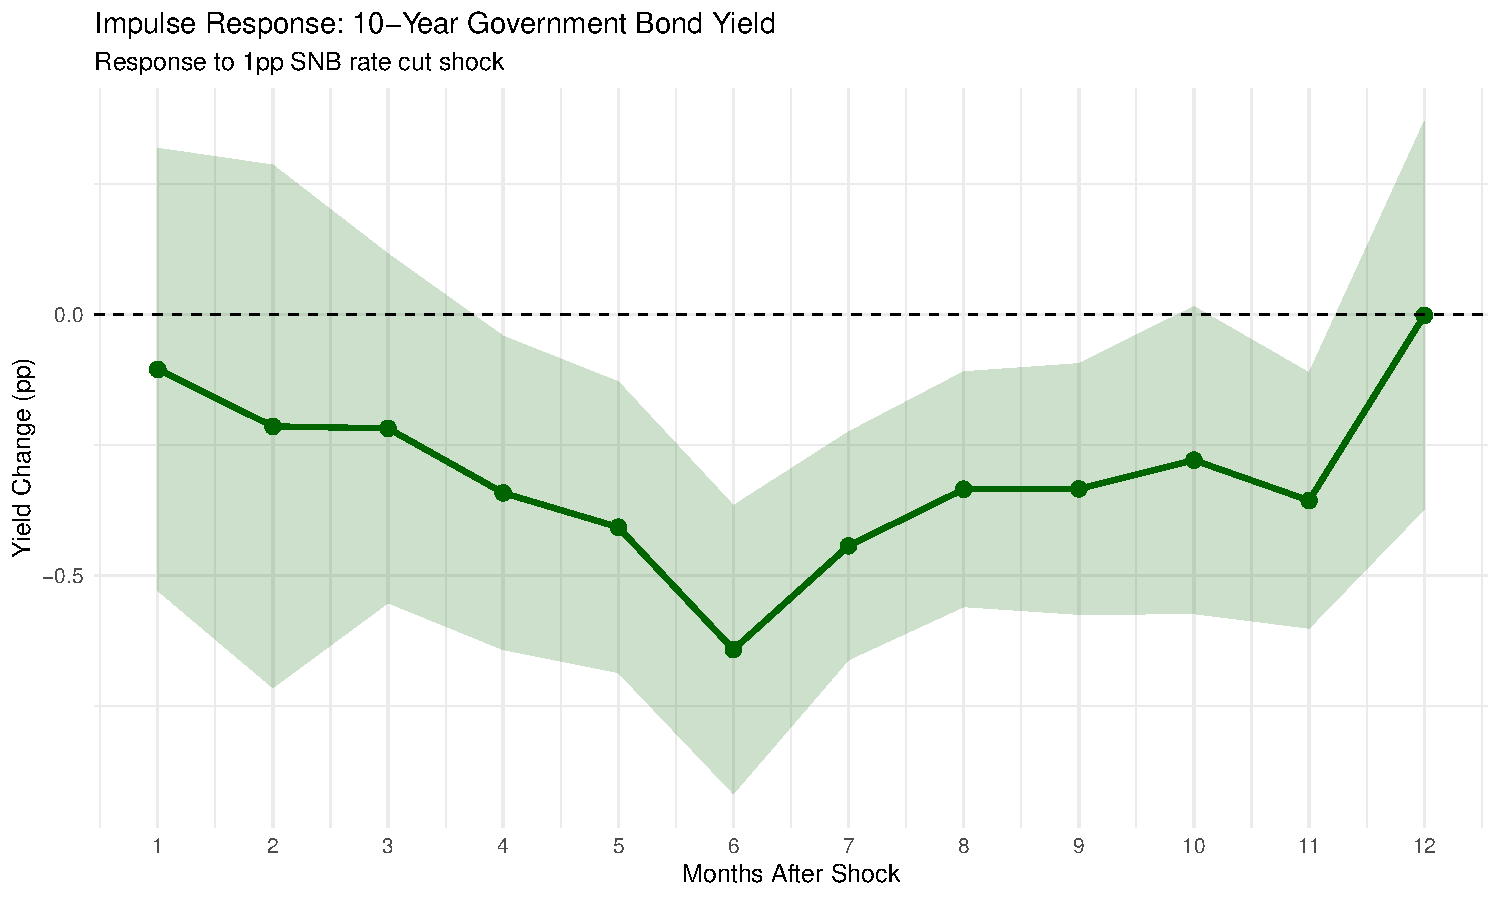
\includegraphics[width=\textwidth]{irf_yield_10y.pdf}
	\caption{Impulse response: 10-year government bond yield.}
	\label{fig:yield10y}
\end{figure}

\begin{figure}[H]
	\centering
	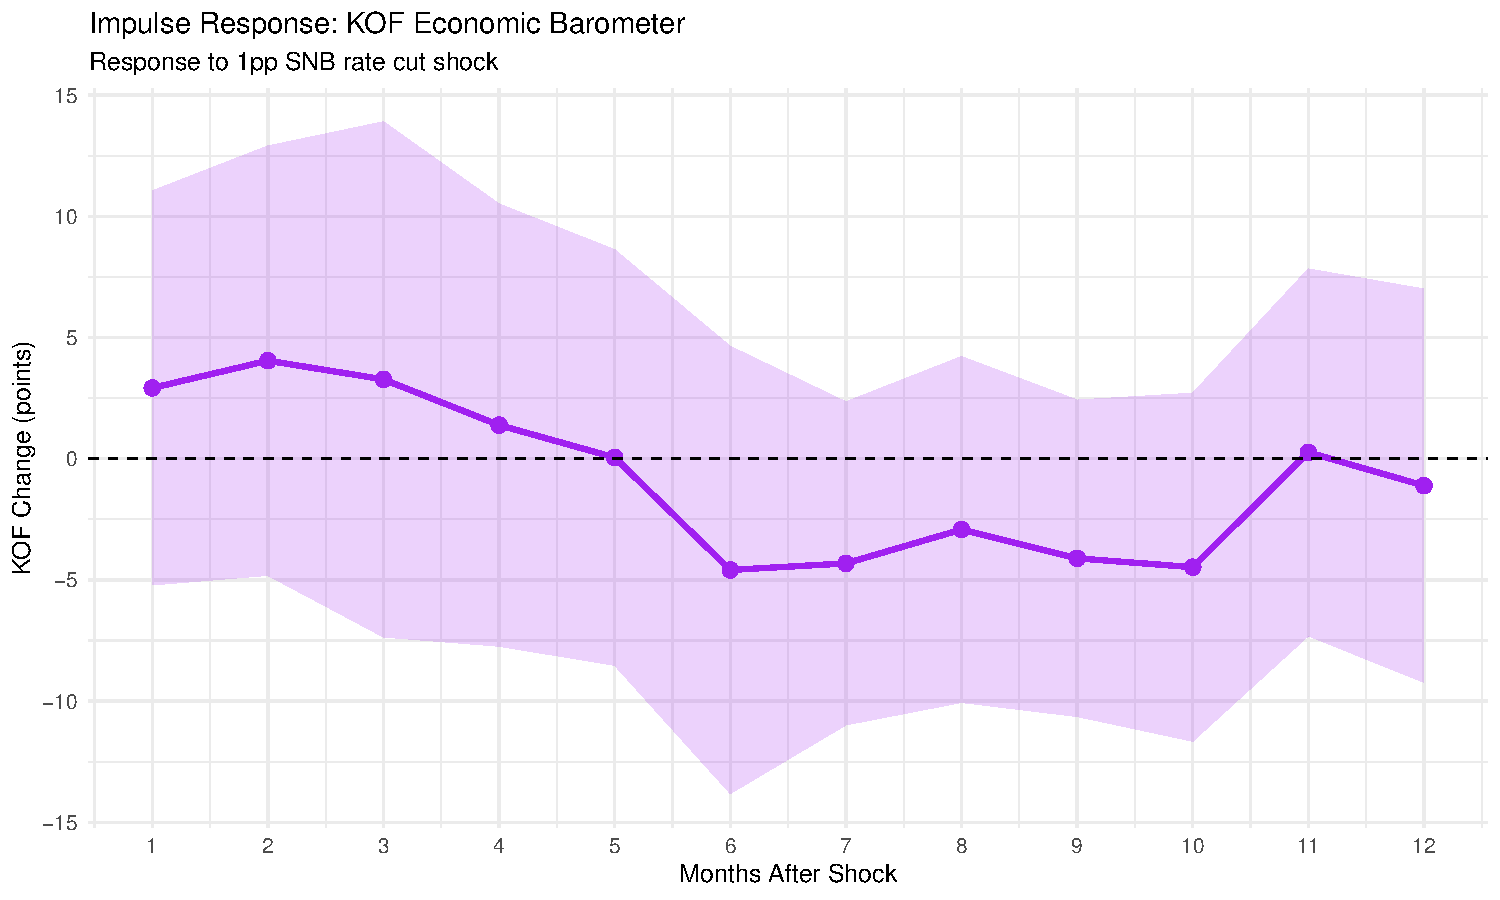
\includegraphics[width=\textwidth]{irf_kof.pdf}
	\caption{Impulse response: KOF Economic Barometer.}
	\label{fig:kof}
\end{figure}

% latex table generated in R 4.5.1 by xtable 1.8-4 package
% Tue Feb 10 16:39:03 2026
\begin{table}[ht]
\centering
\caption{Additional Outcome Variables: LP Impulse Responses to 1pp Rate Cut} 
\label{tab:additional_outcomes}
\begin{tabular}{lrrrr}
  \toprule
Outcome & h = 1 & h = 3 & h = 6 & h = 12 \\ 
  \midrule
2-Year Government Bond Yield & 0.119 (0.115) & -0.199 (0.207) & -0.390 (0.247) & 0.290 (0.276) \\ 
  10-Year Government Bond Yield & -0.106 (0.216) & -0.219 (0.170) & -0.643*** (0.141) & -0.002 (0.189) \\ 
  KOF Economic Barometer & 2.919 (4.148) & 3.273 (5.424) & -4.591 (4.707) & -1.113 (4.141) \\ 
   \bottomrule
\end{tabular}
\end{table}


\subsection{Discussion}

The yield responses trace the term structure channel of monetary policy transmission and produce the most statistically clear-cut result among the additional outcomes.

The 2-year yield response is initially positive ($+0.119$ pp at $h=1$, insignificant) before turning negative ($-0.199$ at $h=3$, $-0.390$ at $h=6$), though it remains statistically insignificant at conventional levels. The initial positive response may seem counterintuitive---a rate cut should lower yields---but is consistent with the information effect channel identified in Section~\ref{sec:info}: if markets interpret the cut as a signal of worse-than-expected economic conditions, short-term yields may temporarily rise as markets reprice risk.

The 10-year yield shows a clear and statistically significant decline of $-0.643$ pp at $h=6$ ($p < 0.01$). This is the only additional outcome with a strongly significant result and has a natural interpretation: rate cuts gradually transmit to longer maturities through the expectations channel, with the full effect materializing at 6 months as markets incorporate the lower policy rate into their long-run interest rate expectations. The effect dissipates by $h=12$ ($-0.002$), suggesting that long yields eventually reflect other macroeconomic developments. The significant 10-year yield decline confirms that SNB rate cuts affect the entire yield curve, not just the short end---a key transmission channel in the DSGE model through the expectations hypothesis.

The KOF barometer responses are economically noisy. The initial positive response ($+2.919$ points at $h=1$) suggests a brief confidence boost, but the large standard error (4.148) renders it insignificant. The reversal at $h=6$ ($-4.591$) and $h=12$ ($-1.113$) may reflect the counter-cyclical nature of rate cuts: they occur during economic weakness, and the KOF barometer may be responding to the underlying economic deterioration that prompted the cut rather than to the monetary stimulus itself. This endogeneity concern illustrates why the purging regression is essential---without removing the systematic component, real activity responses conflate the cause (monetary easing) with the trigger (economic weakness).

\textbf{Implications for RQ2:} The significant 10-year yield decline at 6 months validates a core prediction of the DSGE model: monetary policy transmits to long-term rates through the expectations channel. The DSGE model predicts that the nominal interest rate declines on impact and returns to steady state within 8--12 quarters; the empirical 6-month peak and subsequent fade is qualitatively consistent with this timing. The insignificant KOF responses highlight a limitation of the empirical approach: real activity effects are difficult to isolate when rate cuts are endogenous to economic conditions, even after purging.


% =========================================================================
% EXTENSION 7: SIZE & SIGN ASYMMETRY
% =========================================================================
\section{Size and Sign Asymmetry Tests}\label{sec:asymmetry}

\subsection{Motivation}

Standard linear LP specifications impose symmetric responses to positive and negative shocks of equal magnitude. However, economic theory suggests several channels through which asymmetries may arise: downward nominal rigidities, different credibility of rate cuts vs.\ hikes, or nonlinear portfolio adjustment effects \citep{tenreyro2016}. For the Swiss case, the CHF's safe-haven status \citep{ranaldo2010} could create asymmetries if rate cuts during stress episodes have different exchange rate effects than rate hikes during normalization periods.

\subsection{Methodology}

\textbf{Sign asymmetry.} We decompose the shock into easing and tightening components:
\begin{equation}
	\Delta y_{t+h} = \beta_h^{\text{cut}} \cdot \text{shock}_t^{-} + \beta_h^{\text{hike}} \cdot \text{shock}_t^{+} + \boldsymbol{X}_t'\boldsymbol{\phi}_h + \varepsilon_{t+h}
\end{equation}
where $\text{shock}_t^{-} = \text{mp\_shock}_t \cdot \mathbf{1}(\text{mp\_shock}_t < 0)$ and $\text{shock}_t^{+} = \text{mp\_shock}_t \cdot \mathbf{1}(\text{mp\_shock}_t > 0)$. A Wald test for $H_0: \beta_h^{\text{cut}} = \beta_h^{\text{hike}}$ assesses symmetry.

\textbf{Size asymmetry.} We split shocks at the median absolute value of nonzero shocks:
\begin{equation}
	\Delta y_{t+h} = \beta_h^{\text{large}} \cdot \text{shock}_t^{L} + \beta_h^{\text{small}} \cdot \text{shock}_t^{S} + \boldsymbol{X}_t'\boldsymbol{\phi}_h + \varepsilon_{t+h}
\end{equation}

\textbf{Quantile regression.} As a robustness check, we estimate quantile regressions at $\tau \in \{0.25, 0.50, 0.75\}$ to characterize the conditional distribution of responses \citep{koenker1978}.

\subsection{Results}

\begin{figure}[H]
	\centering
	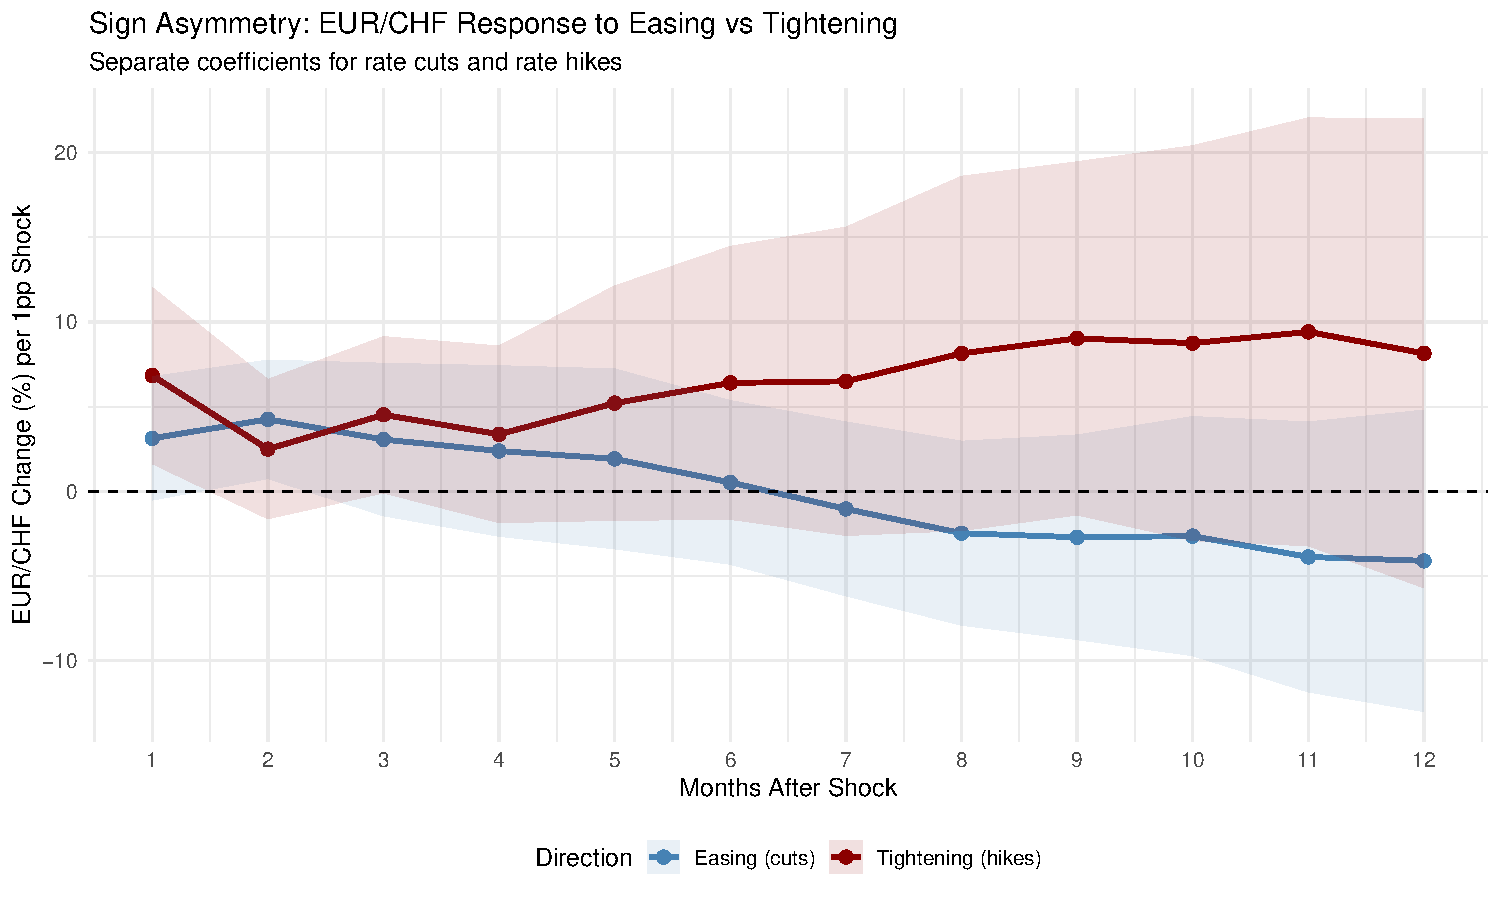
\includegraphics[width=\textwidth]{irf_sign_asymmetry_fx.pdf}
	\caption{Sign asymmetry: EUR/CHF response to rate cuts (easing) vs.\ rate hikes (tightening).}
	\label{fig:sign_asym}
\end{figure}

\begin{figure}[H]
	\centering
	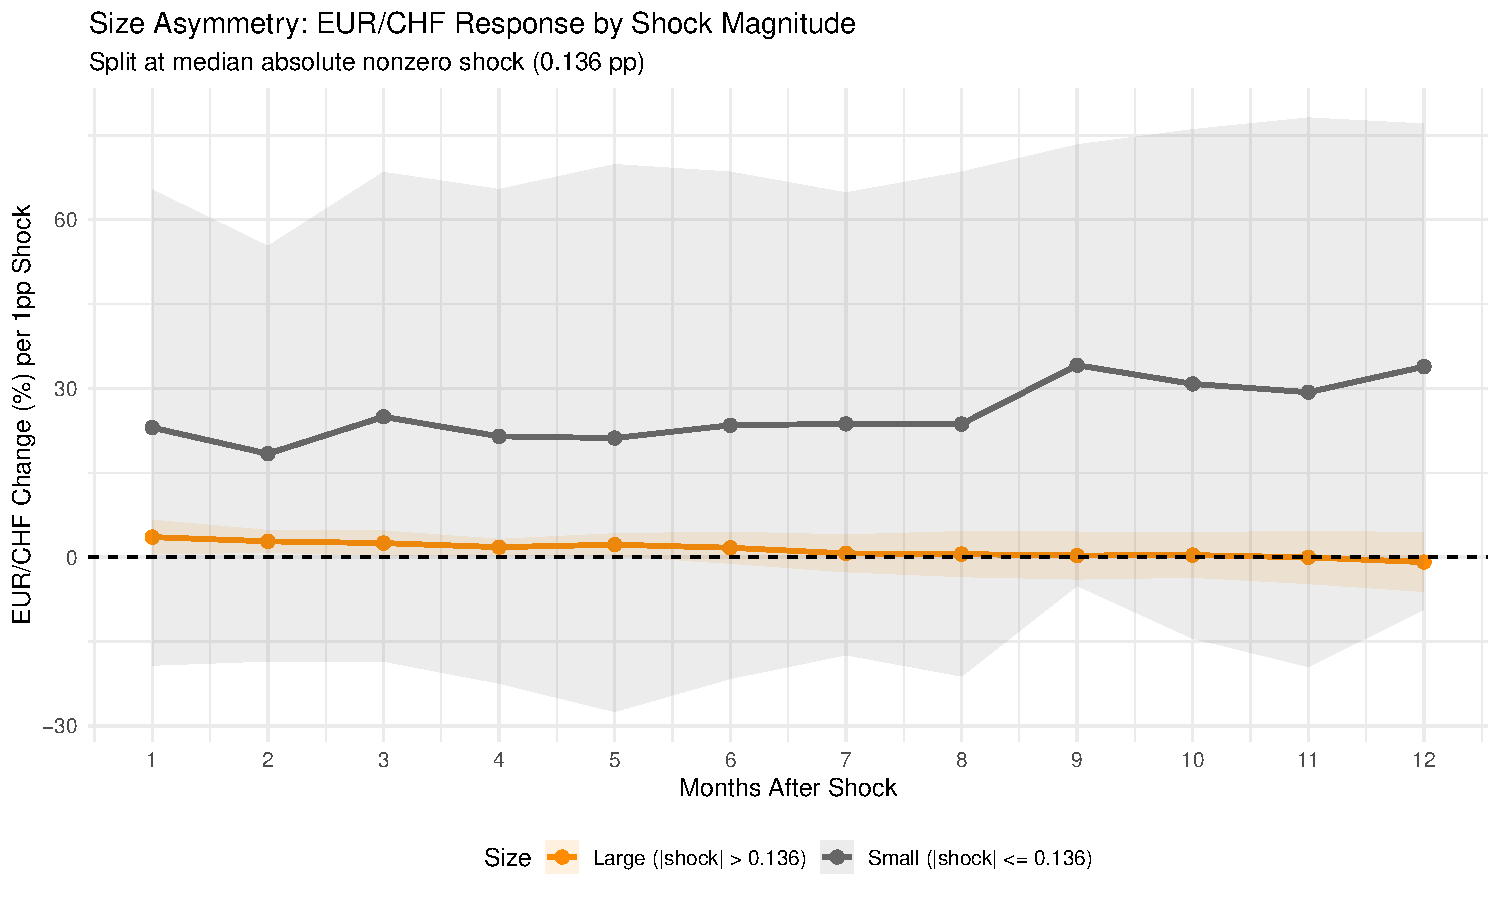
\includegraphics[width=\textwidth]{irf_size_asymmetry_fx.pdf}
	\caption{Size asymmetry: EUR/CHF response to large vs.\ small shocks.}
	\label{fig:size_asym}
\end{figure}

% latex table generated in R 4.5.1 by xtable 1.8-4 package
% Tue Feb 10 09:12:47 2026
\begin{table}[ht]
\centering
\caption{Asymmetry Tests: EUR/CHF Response by Shock Sign and Size} 
\label{tab:asymmetry_results}
\begin{tabular}{crrrrrr}
  \toprule
h & Cuts & Hikes & Sign Wald & Large & Small & Size Wald \\ 
  \midrule
  1 & 3.13* (1.86) & 6.83** (2.65) & 1.08 [0.300] & 3.56** (1.54) & 23.04 (21.56) & 0.79 [0.375] \\ 
    3 & 3.06 (2.30) & 4.52* (2.35) & 0.14 [0.711] & 2.50** (1.11) & 24.96 (22.18) & 1.01 [0.316] \\ 
    6 & 0.53 (2.46) & 6.40 (4.11) & 0.94 [0.334] & 1.67 (1.42) & 23.45 (22.98) & 0.86 [0.354] \\ 
   12 & -4.10 (4.54) & 8.14 (7.06) & 1.25 [0.265] & -0.88 (2.67) & 33.88 (22.01) & 2.31 [0.130] \\ 
   \bottomrule
\end{tabular}
\end{table}


% latex table generated in R 4.5.1 by xtable 1.8-4 package
% Tue Feb 10 09:29:09 2026
\begin{table}[ht]
\centering
\caption{Quantile Regression: EUR/CHF Response at Different Quantiles} 
\label{tab:quantile_regression}
\begin{tabular}{crrr}
  \toprule
horizon & tau = 0.25 & tau = 0.5 & tau = 0.75 \\ 
  \midrule
1.00 & 2.04 (5.90) & 3.04*** (0.95) & 3.14 (2.21) \\ 
  3.00 & 2.29 (4.53) & 1.24 (1.89) & 0.44 (5.77) \\ 
  6.00 & -3.81 (3.37) & 0.49 (2.00) & 3.64** (1.56) \\ 
  12.00 & -6.59 (4.58) & -1.26 (3.98) & 3.63 (5.91) \\ 
   \bottomrule
\end{tabular}
\end{table}


\subsection{Discussion}

Neither sign nor size asymmetry is statistically significant at any horizon, with all Wald $p$-values exceeding 0.10. This is an important non-result that constrains the interpretation of the main findings.

For sign asymmetry, rate hikes generate numerically larger point estimates than rate cuts at short horizons (6.83 vs.\ 3.13 at $h=1$), but the Wald test fails to reject equality ($p = 0.300$). The larger hike coefficients could reflect the safe-haven channel: SNB tightening during normalization may trigger CHF appreciation as carry trade positions unwind, amplifying the exchange rate response relative to cuts during stress. However, the wide confidence intervals---driven by few hike observations---preclude strong conclusions. At longer horizons, both estimates lose significance and the Wald tests remain firmly insignificant ($p = 0.265$ at $h=12$).

For size asymmetry, large shocks produce stable, precisely estimated effects (3.56 at $h=1$, significant at 5\%), while small shocks yield enormous but wildly imprecise point estimates (23.04 at $h=1$). The very large small-shock coefficients are an artifact of the scaling: small shocks by definition have near-zero magnitude, so even modest exchange rate movements translate into large per-unit coefficients. The Wald tests correctly identify that this apparent difference is not statistically meaningful ($p = 0.375$).

The quantile regression results reveal interesting distributional heterogeneity. At $h=1$, the median response (3.04, significant at 1\%) is well-estimated, while the lower (2.04) and upper (3.14) quartile responses have wider confidence intervals. At $h=6$, the upper quartile shows a significant response (3.64, $p < 0.05$) while the lower quartile is insignificant, suggesting that the exchange rate response is stronger in episodes where the franc depreciates more broadly---consistent with safe-haven unwinding during calmer market conditions.

\textbf{Implications for RQ1:} The absence of significant asymmetry supports the linear specification used in the main analysis. The main thesis's finding of 4.5\% depreciation per pp shock appears to apply symmetrically to cuts and hikes, large and small shocks, justifying the pooled estimation. This also distinguishes the sign/size asymmetry (not found) from the regime asymmetry (strongly significant in the main thesis), suggesting that regime dependence operates through structural changes in the transmission mechanism (e.g., the 2015 floor removal) rather than through nonlinear responses to shock characteristics.


% =========================================================================
% CONCLUSION
% =========================================================================
\section{Conclusion}\label{sec:conclusion}

The seven extensions presented in this document strengthen and extend the main thesis analysis along three dimensions, with direct implications for both research questions.

\textbf{Identification.} The high-frequency IV approach (Section~\ref{sec:hf}) highlights the limitations of small-sample IV estimation with only 25 events, confirming that the purging regression remains the most feasible identification strategy with available data. The information effect decomposition (Section~\ref{sec:info}) reveals that pure monetary shocks generate a 4.3\% exchange rate depreciation and near-zero CPI effects---closely matching the DSGE model's predictions and suggesting that the baseline pooled estimates blend pure policy with information channels.

\textbf{Inference.} The wild bootstrap (Section~\ref{sec:bootstrap}) confirms the impact exchange rate effect ($p = 0.025$) but suggests that persistence beyond 1 month is less robust than Newey-West inference indicates ($p = 0.128$ at $h=3$). The placebo tests (Section~\ref{sec:placebo}) provide the strongest validation of the identification strategy: anticipated policy produces no exchange rate response, and the actual shock effect is significant in only 1.8\% of random permutations at $h=1$. Together, these results narrow the main thesis's finding from ``significant depreciation through 6 months'' to ``robust impact depreciation with suggestive persistence.''

\textbf{Heterogeneity.} The smooth transition framework (Section~\ref{sec:smooth}) confirms stable normal-rate transmission ($\sim$4.2\% depreciation) but shows that low-rate estimates are sensitive to the transition specification, reinforcing the main thesis's cautious interpretation of regime differences. Additional outcome variables (Section~\ref{sec:outcomes}) reveal a significant 10-year yield decline at 6 months, validating the DSGE model's expectations channel. The absence of sign and size asymmetry (Section~\ref{sec:asymmetry}) supports the linear LP specification and distinguishes structural regime dependence from nonlinear shock responses.

Taken together, these extensions support the core conclusions of the main thesis while refining their precision. The most robust finding across all methods is the immediate exchange rate depreciation of approximately 4--5\% per percentage point rate cut shock, significant under asymptotic inference, wild bootstrap, and permutation tests. The weak inflation response to pure monetary shocks validates the DSGE model's incomplete pass-through mechanism. The regime-dependent results remain statistically significant but should be interpreted as reflecting the extraordinary 2015 floor removal episode rather than a general property of monetary transmission under negative interest rates.


% =========================================================================
% BIBLIOGRAPHY
% =========================================================================
\newpage
\bibliography{ref_ext}

\end{document}
